% debut d'un fichier latex standard
\documentclass[a4paper,12pt,twoside]{article}

% Pour les unités SI
\usepackage{siunitx}

% Déclaration de l'unité "radian"
%\DeclareSIUnit{\rad}{\milli\meter\textrm{-}\milli\radian}

% pour l'inclusion de figures en eps,pdf,jpg
\usepackage{graphicx}
% quelques symboles mathematiques en plus
\usepackage{amsmath}
% le tout en langue francaise
%\usepackage[english]{babel}
% on peut ecrire directement les caracteres avec l'accent
% a utiliser sur Linux/Windows
\usepackage[utf8]{inputenc}
\usepackage[T1]{fontenc}

% pour faire des systèmes d'équations
\usepackage{systeme}
\setcounter{tocdepth}{3} % Augmente le niveau affiché dans la table des matières

% a utiliser sur le Mac
%\usepackage[applemac]{inputenc}
% pour l'inclusion de links dans le document
\usepackage[colorlinks,bookmarks=false,linkcolor=blue,urlcolor=blue]{hyperref}
\usepackage{subcaption}
\paperheight=297mm
\paperwidth=210mm

\setlength{\textheight}{235mm}
\setlength{\topmargin}{-1.2cm} % pour centrer la page verticalement
%\setlength{\footskip}{5mm}
\setlength{\textwidth}{15cm}
\setlength{\oddsidemargin}{0.56cm}
\setlength{\evensidemargin}{0.56cm}

\pagestyle{plain}

% quelques abreviations utiles
\def \be {\begin{equation}}
\def \ee {\end{equation}}
\def \dd  {{\rm d}}

\newcommand{\mail}[1]{{\href{mailto:#1}{#1}}}
\newcommand{\ftplink}[1]{{\href{ftp://#1}{#1}}}
%
% latex SqueletteRapport.tex      % compile la source LaTeX
% xdvi SqueletteRapport.dvi &     % visualise le resultat
% dvips -t a4 -o SqueletteRapport.ps SqueletteRapport % produit un PostScript
% ps2pdf SqueletteRapport.ps      % convertit en pdf

% pdflatex SqueletteRapport.pdf    % compile et produit un pdf


% ======= Le document commence ici ======

\begin{document}
% Le titre, l'auteur et la date
\title{Exercise 3: Pendulum with a vertical excitation\\{\small Physique Numérique I}}
\date{\today}
\author{Delphine Martres et Damien Korber\\{\small \mail{delphine.martres@epfl.ch} et \mail{damien.korber@epfl.ch}}}
\maketitle
\tableofcontents % Table des matieres
\newpage % Si la toc est trop grande, voir ligne 19.
% Quelques options pour les espacements entre lignes, l'identation
% des nouveaux paragraphes, et l'espa	cement entre paragraphes
\baselineskip=16pt
\parindent=15pt
\parskip=5pt



%%%% ON COMMENCE A ECRIRE D'ICI

\section{Introduction}
%TODO : Améliorer cette impro.
This experiment will focus on the study of a simple pendulum in a box moving with a certain frequency.
This allows a study of different situation, one of whom is the study of chaotic movements.

\section{Analytical computations}
%TODO : Revoir en détail cette partie: Y'a eu l'ajout de la boîte entre deux, donc il faut vérifier que tout soit encore d'actualité.
\subsection{Differential equation of the problem}
After some computations described in appendix \ref{ann:eq-diff}, equation \ref{eq:equa-diff} results.%TODO : Faire l'annexe en question.

\begin{equation}
	\ddot{\theta} = -\frac{\kappa}{m}\dot{\theta} - \frac{g}{L}\sin\theta
	\label{eq:equa-diff}
\end{equation}
where $\kappa$ is an air resistance coefficient, $m$ is the mass, $\theta$ is the angle of the pendulum, $g$ the mean gravity on earth and $L$ the length of the rod.

Equation \ref{eq:equa-diff} can also be written as equation \ref{eq:equa-diff-sys}, which is better for numerical computations.

\begin{equation}
	\frac{d}{dt}
	\begin{pmatrix}
		\theta \\ \dot{\theta}
	\end{pmatrix}
	= \begin{pmatrix}
	\dot{\theta} \\
		-\frac{\kappa}{m}\dot{\theta} - \frac{g}{L}\sin\theta
	\end{pmatrix}
	\label{eq:equa-diff-sys}
\end{equation}

\subsection{Mechanical energy and power of non-conservative forces in the frame of reference $R'$}
The only energy to consider is the kinetic energy of rotation, and the potential energy, as there is no translation.
The kinetic energy of rotation is given by $E_{c,r} = \frac{1}{2}I\omega^2$, where $I$ is the moment of inertia and $\omega$ the angular velocity.
The moment of inertia of a solid can be tough to compute for generic objects, but for a discrete number of masses, the moment of inertia is given by equation \ref{eq:moment-inertie}. \cite{ans:moment-inertie} %TODO : Ajouter à la bibliographie le livre de meca pour la formule de I.

\begin{equation}
	I = \sum_\alpha m_\alpha r_\alpha^2
	\label{eq:moment-inertie}
\end{equation}
where $m_\alpha$ is the mass and $r_\alpha$ is the distance between the origin considered and the mass.

In the case of the pendulum, it is quite trivial to compute.
The mass of rod of the pendulum is ignored, and the mass $m$ of the pendulum is condensed in a single point at a distance $L$ of the origin of $R'$.

The moment of inertia is given by $I=mL^2$.\\ %TODO : J'ai pas trouvé de traduction de "point matériel".

The mechanical energy is then expressed as equation \ref{eq:emec}.

\begin{equation}
	E_m = \frac{1}{2}I\omega^2 - mgL\cos\theta =  \frac{mL^2}{2}\dot{\theta}^2 - mgL\cos\theta
	\label{eq:emec}
\end{equation}

Regarding the power, there is only one force to consider, the air resistance (or drag), because it is the only non-conservative one.
The power is expressed as $P = \mathbf{F}\cdot\mathbf{v}$, and the drag is defined as $\mathbf{f} = -\kappa\mathbf{v'}$ in this report, where $\mathbf{v'}$ is the speed in the frame of reference $R'$.
These vectors are given by:

\begin{align*}
	\mathbf{f} =
	\begin{pmatrix}
		f\cos\theta \\
		f\sin\theta \\
		0
	\end{pmatrix}
	= \begin{pmatrix}
		f\cos\theta \\
		f\sin\theta \\
		0
	\end{pmatrix}
	\text{ and }
	\mathbf{v} =
	\begin{pmatrix}
		-v'\cos\theta \\
		-v'\sin\theta \\
		0
	\end{pmatrix}
	= \begin{pmatrix}
		-\dot{\theta}L\cos\theta \\
		-\dot{\theta}L\sin\theta \\
		0
	\end{pmatrix}
\end{align*}

The power of the drag is then given by equation \ref{eq:power}.
\begin{equation}
	P = \kappa\dot{\theta}^2 L^2
	\label{eq:power}
\end{equation}


\subsection{Solutions for little movements around equilibrium}\label{sec:sol-analytique}
%TODO : à remplir
%TODO : Mettre la solution analytique finale avec eq:sol-analytique-gen comme label.
\section{Numerical computations}

Unless specified otherwise, all simulations are done using a time step of $\Delta t = \SI{2d-2}{\s}$.

\subsection{Little movements without excitation or air resistance}
In this section, no excitation or air resistance will be considered: $\kappa = 0$, $d = 0$.
The movements are small, such that approximations are made: $\theta_0 = \num{d-6}$, $\dot{\theta}_0 = 0$.
The simulation runs for \SI{20}{\second}.

\subsubsection{Comparison between the analytical solution and the approximation of Stormer-Verlet method}
The problem is easy enough to be able to compute the analytical solution.
The general solution is given in section \ref{sec:sol-analytique} by equation \ref{eq:sol-analytique-gen}.
Using the defined initial conditions, the constants can be computed, and the analytical solution for this problem is given by equation \ref{eq:a-sol-ana}.

\begin{equation}
	\theta = 10^{-6}\cos(\omega_0t)
	\label{eq:a-sol-ana}
\end{equation}

It is then possible to compare the analytical solution with the results found using the numerical method of Stormer-Verlet, which is done in figure \ref{fig:a-traj}.

\begin{figure}[h]
\centering
\begin{subfigure}[t]{0.45\textwidth}
	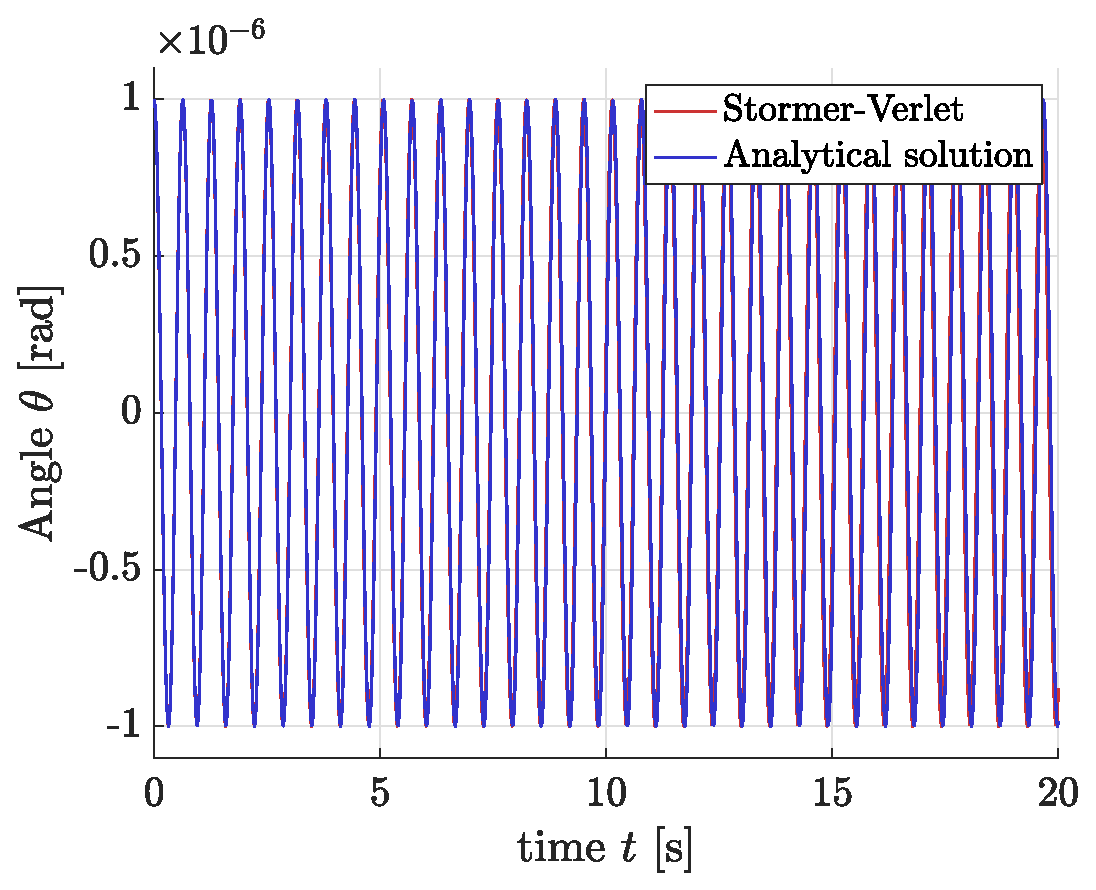
\includegraphics[width=\textwidth]{graphs/a_traj_full.eps}
	\caption{Angle of the pendulum with respect to time, with a comparison between the Stormer-Verlet numerical method and the analytical solution.}
	\label{fig:a-traj-full}
\end{subfigure}
~
\begin{subfigure}[t]{0.45\textwidth}
	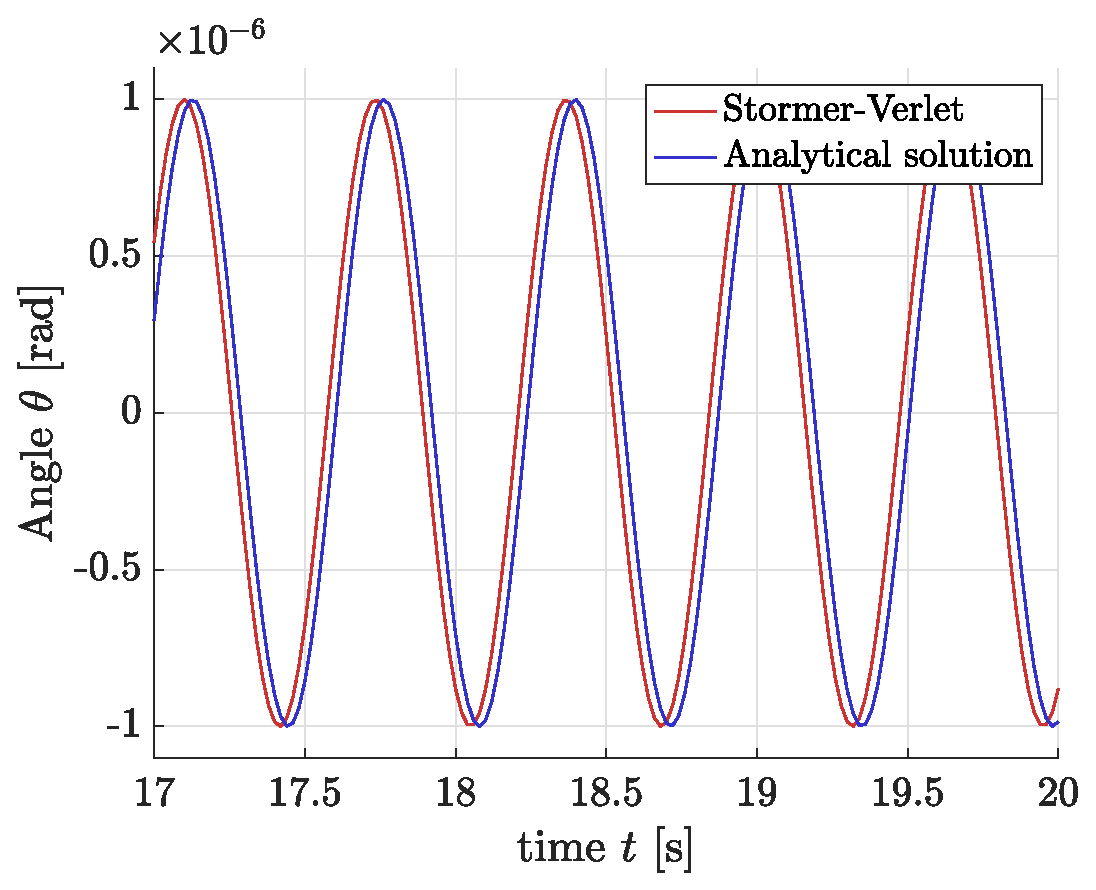
\includegraphics[width=\textwidth]{graphs/a_traj_zoomed.eps}
	\caption{Same plot as \ref{fig:a-traj-full}, with the beginning cropped out to get a better view of the small difference between the numerical and analytical solutions at the end of the simulation.}
	\label{fig:a-traj-zoomed}
\end{subfigure}
\caption{Angle of the pendulum with respect to time, using Stormer-Verlet numerical method at \num{1000} steps and the analytical solution.}
\label{fig:a-traj}
\end{figure}

Figure \ref{fig:a-traj-full} shows a comparison of Stromer-Verlet's numerical method and the analytical solution.
Those plots almost overlap, and the numerical method seems quite accurate knowing the small number of steps considered.
The numerical method seems to be stable over time.
Figure \ref{fig:a-traj-zoomed} shows the same comparison, but focuses on the end of the simulation, where the peak difference occurs.
This slight difference does not seem to affect the amplitude of the sinus, but only its period.
The numerical method has a slightly decreasing period over time.
This comes from computational errors and not from the numerical method, as Stormer-Verlet seems to be stable in this problem.
These errors are probably generated when numbers are rounded.
%TODO : Vraiment (pour les 2 dernières lignes) ? Vérifier avec le rapport de la dernière fois, parce qu'il me semble qu'on a déjà dit un truc similaire (et faux).
%TODO : Les 2-3 dernières phrases me semblent assez moche, faudrait les modifier.


\subsubsection{Convergence study}
In this section, the convergence of the numerical method of Stormer-Verlet will be studied.

\begin{figure}[h]
\centering
	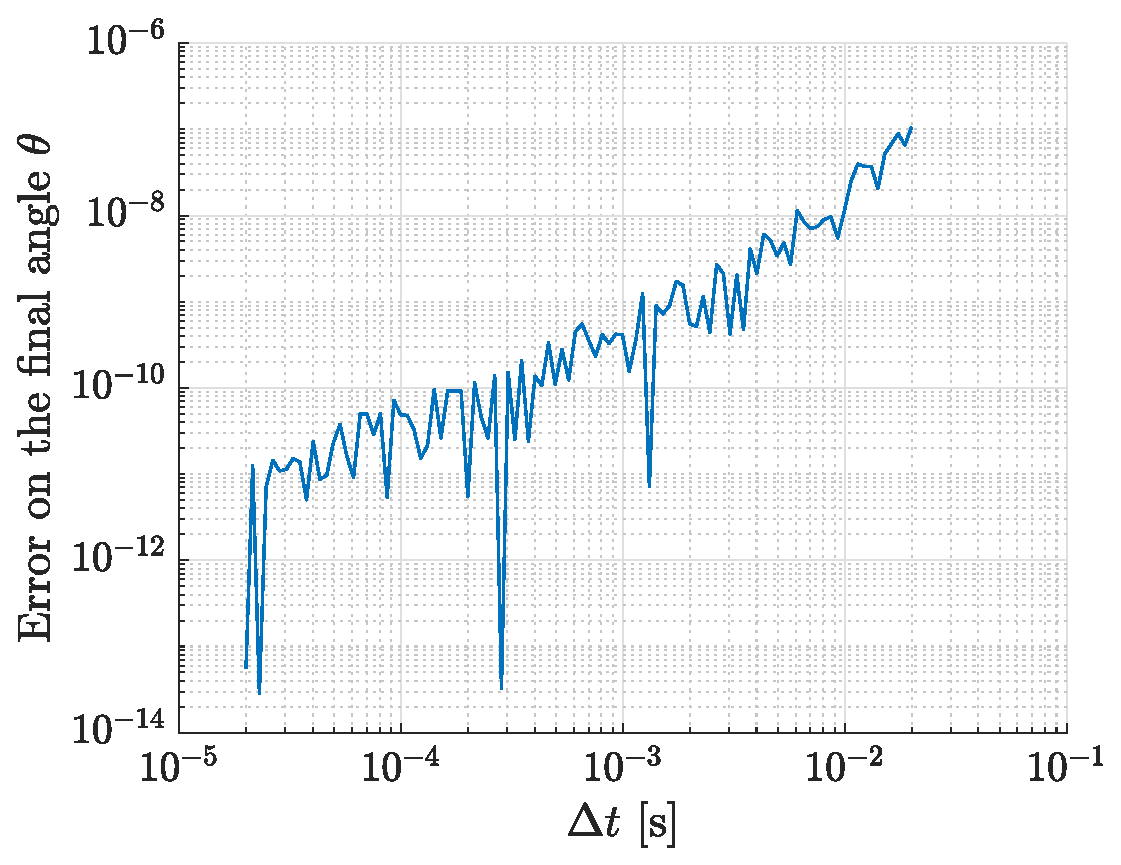
\includegraphics[width=0.6\textwidth]{graphs/a_conv.eps}
	\caption{Error on the final angle of the pendulum with respect to the time step. The final time is not exactly \SI{20}{\s} for every case, but is often a close value, which is the final time, but of the sum of some $\Delta t$ do not end on \num{20}. \num{20} simulations are considered in this study.} %TODO : Je trouve la dernière phrase pas très belle. Si t'as une amélioration, je suis preneur.
	\label{fig:a-conv}
\end{figure}

Figure \ref{fig:a-conv} show the study of the error the final angle with respect to the time step.
The main aspect of this study is the order of convergence of Stormer-Verlet's method.
On a log-log graph, the error decreases linearly with smaller time steps.
By finding the slope of the drawn line, the order of Stormer-Verlet's method can be deduced.
The numerical scheme of Stormer-Verlet is defined as an order-2 numerical method, which is verified on this figure.
The slope of the line is 2, which implies a second order numerical method.
This implies that, when the time step $\Delta t$ is divided by \num{10}, the error is divided by \num{100}.
For example, in this simulation, when $\Delta t = \num{d-2}$, the error is of order \num{d-8} and when $\Delta t = \num{d-3}$, the error is of order \num{d-10}, which is a division by \num{100}.
%TODO : Idée: Parler de la taille des erreurs. Grand ? Petit ?

In summary, the numerical method of Stormet-Verlet converges.
%TODO : Il faut refaire cette section (c'est la version sur l'ancien graph, donc plus actuel.) -> DONE. TO BE ERASED.
% Ce que je veux dire: L'erreur est divisée par 100 quand le time step est divisé par 10, le fait que le résultat converge parce que ça descend linéairement sur le graph (log), et parler de l'ordre de grandeur de l'erreur.
%Figure \ref{fig:a-conv} shows the convergence study of this problem.
%The first point to verify is the convergence order of the numerical method.
%In this figure, the curve follows an almost constant linear decrease (with a log scale).
%On this plot, dividing the time step by \num{10} almost divides the error by \num{100}.
%This implies a second order numerical method: when the time step is divided by any number $h$, the error is divided by $h^2$.
%For example, at $\Delta t = \SI{d-2}{\second}$ the error is estimated by $err = \num{d-8}$.
%By dividing by \num{10} the time step ($\Delta t = \SI{d-3}{\second}$), the error is now estimated by $err \approx \num{d-10}$, which is \num{100} times smaller.\par
%The second point how small the error gets.
%Consider that the final angle is of order \num{d-6} (fig. \ref{fig:a-traj-full}).
%When the time step is big, $\Delta t = \SI{d-2}{\second}$ for example, the error reaches \SI{10}{\percent}.
%Computations are quite fast and easy to do at this time step.
%Just by lowering a little the time step, the error easily gets smaller that \SI{1}{\percent} or even less, which is gives a good approximation of the problem.
%In summary, Stormer-Verlet's numerical method converges fast, and is fits well the problem in term of convergence.


\subsubsection{Conservation of energy}

\begin{figure}[h]
\centering
	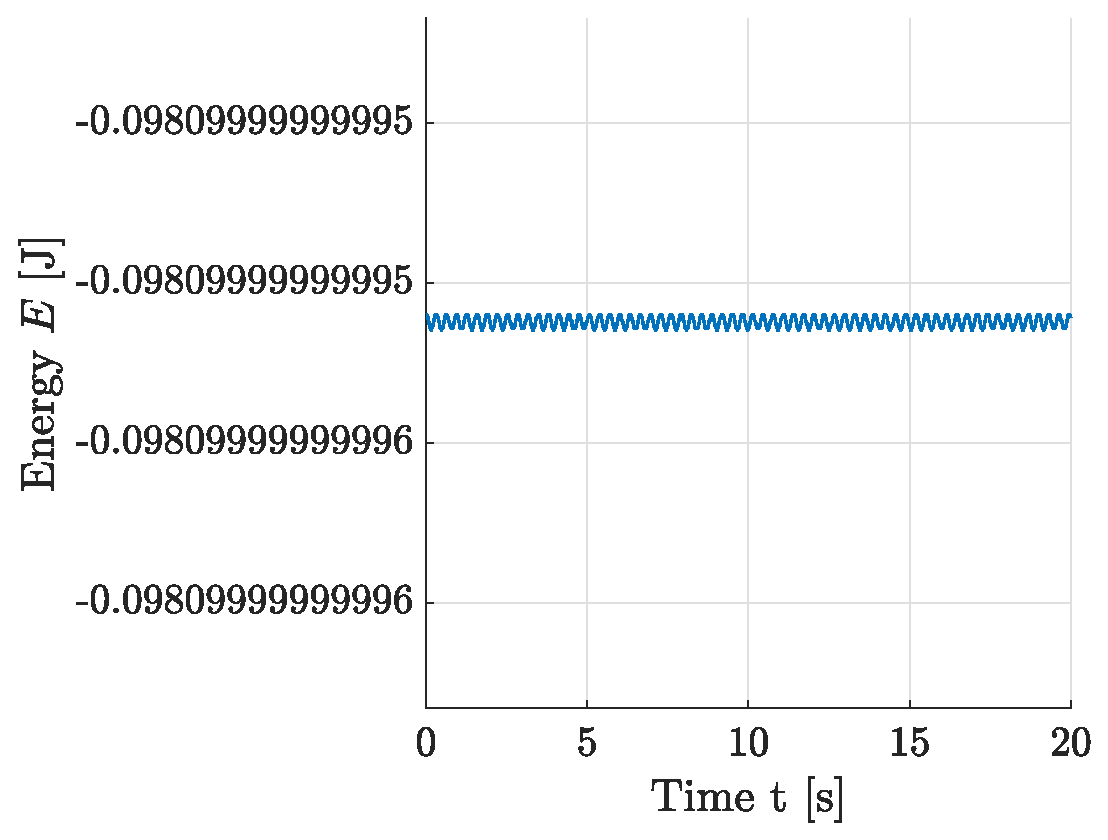
\includegraphics[width=0.6\textwidth]{graphs/a_ener.eps}
	\caption{Study of the mechanical energy of the pendulum with respect to time. The time step used is $\Delta t = \SI{2d-2}{\s}$.}
	\label{fig:a-ener}
\end{figure}

%Ce que je veux dire: L'énergie n'est pas conservée à cause des oscillations, le fait que la variation est très petite sur un nombre pas si petit,  que l'énergie est conservée en moyenne car c'est un schéma symplectique.
Figure \ref{fig:a-ener} shows a study of the mechanical energy over time.
The first information to notice is that mechanical energy does not seem to be conserved even though it should be.
Energy does little oscillations around a line, but does not follow a linear curve.
However, these variations are really small compared to the energy.
The order of magnitude of the energy is \SI{100}{\milli\joule}, where the order of magnitude of the variation of energy is \SI{100}{\pico\joule}. %TODO : Vérifier que ce soit juste. (c'est assez difficile à voir à l'oeil nu)
The variation is so small that it could be easily ignored, and the energy is considered as conserved.
Furthermore, Stormer-Verlet is a symplectic numerical method, which is shown in this figure.
The energy does not grow over time, it is bounded.
The mean mechanical energy is then conserved over time, which implies that, even if the energy is not fully conserved, the numerical method could still be used, as the error would not explode. %TODO : Remplacer 'explode' %TODO : Est-ce qu'on fait une régression linéaire dans ce graph ? Pour montrer que c'est conservé en moyenne.


\subsection{Great movements: period with respect to amplitude}

\begin{figure}[h]
\centering
\begin{subfigure}[t]{0.45\textwidth}
	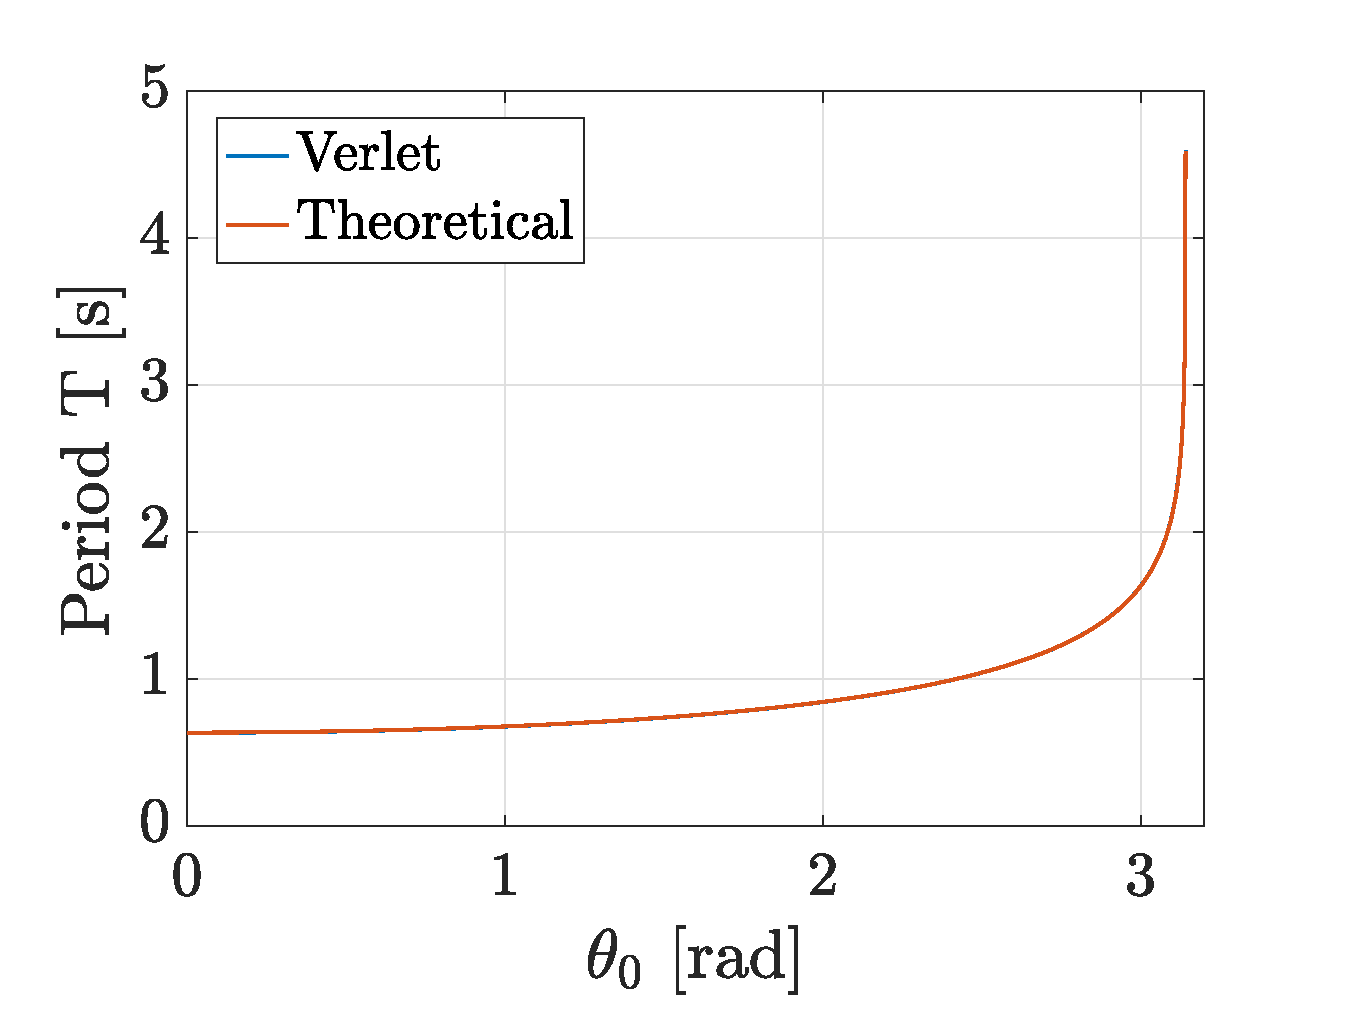
\includegraphics[width=\textwidth]{graphs/b_period.eps}
\end{subfigure}
~
\begin{subfigure}[t]{0.45\textwidth}
	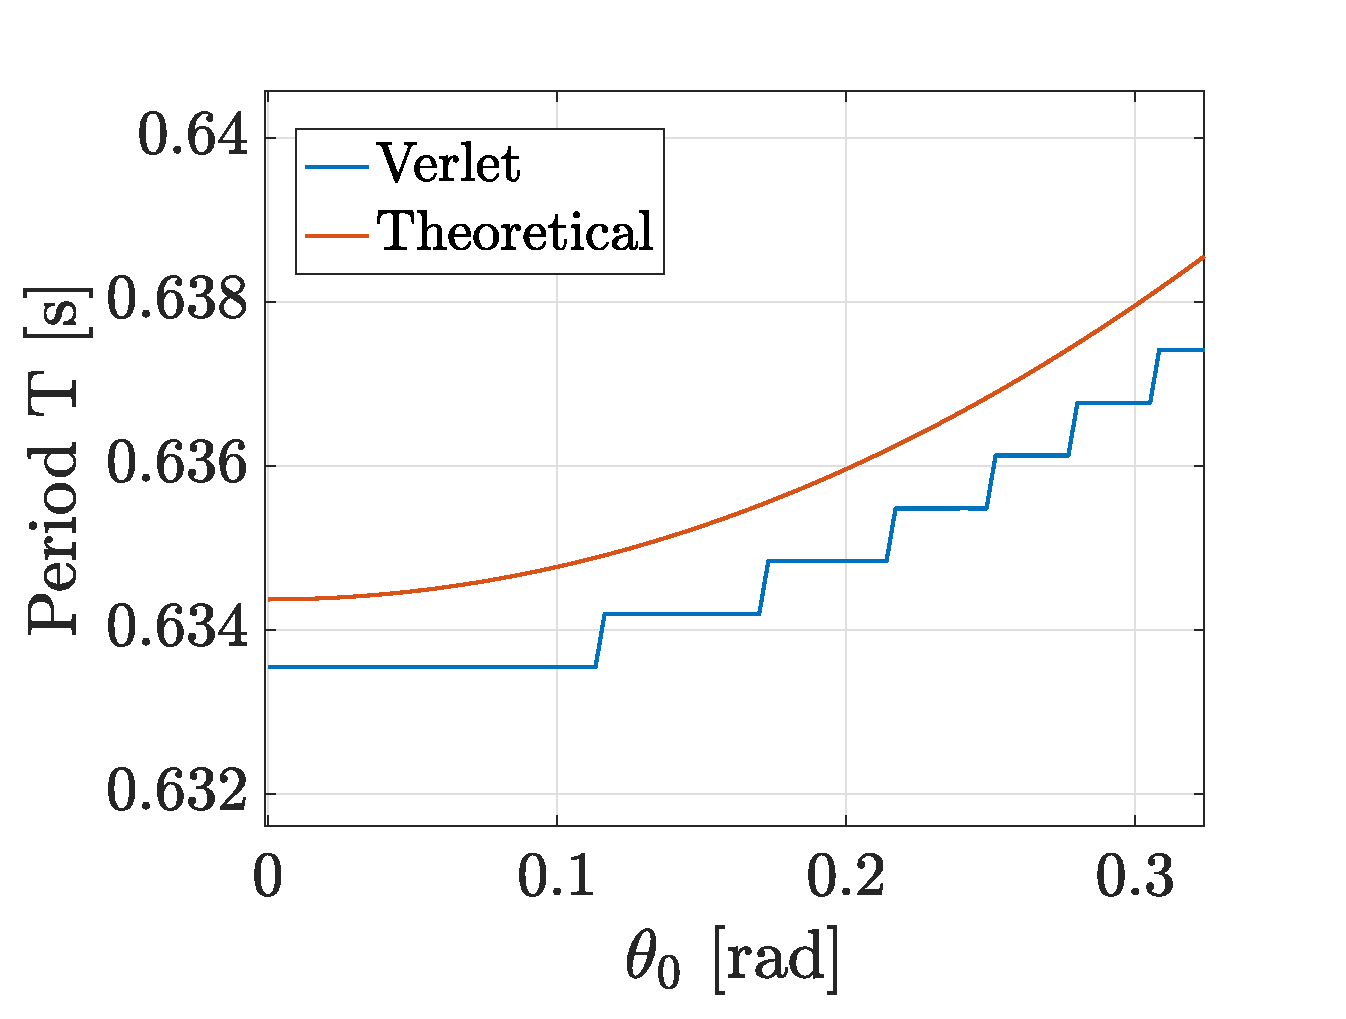
\includegraphics[width=\textwidth]{graphs/b_period_zoom.eps}
\end{subfigure}
\caption{Period of the pendulum with the amplitude $\theta_0 \in ]0,\pi[$ (zoomed in on the right-hand side graph), computed over \num{1000} simulations.}
\label{fig:b-period}
\end{figure}

The period of the pendulum was measured over $1000$ simulations with $\theta_0 \in ]0,\pi[$, using the Verlet method, and the resulting plot is shown on figure \ref{fig:b-period}, compared to the analytical solution. As expected, the period grows exponentially with respect to the amplitude.

The difference between the simulation and the theoretical solution is only visible on the zoomed graph, wherein we see that it is of order $10^{-4}$ at this point of the graph. Only part of the graph is shown on the zoomed-in figure, but the two lines stay no less close all throughout and sometimes cross over each other. It is apparent however that the plot showing the Verlet simulations' periods is not as smooth as the theoretical line, as it has a stair-like shape. Overall this comparison shows that the Verlet method has a good precision. %TODO : Faut peut-être parler de l'ordre de grandeur de la différence.

%%%%%%%%%%%%%%%%%%%%%%%%%%%%%%%%%

\subsection{Resonant excitation}

In this section, the box does move, which implies an external excitation on the pendulum.
The initial conditions are given by $\theta_0 = \SI{0}{\radian}$ and $\dot{\theta} = \SI{d-2}{\radian\per\second}$.
The constants are given by $\Omega = \omega_0$, $d = \SI{3d-2}{\m}$, $\kappa = \SI{0}{\kg\per\s}$ and $t_{end} = \SI{250}{\s}$.

\subsubsection{Verification of the mechanical energy theorem}\label{sec:c-thm}
The mechanical energy theorem is given by equation \ref{eq:thm-ene}. \cite{wiki:en-cin}

\begin{equation}
	\frac{dE_m}{dt} = P_{nc}
	\label{eq:thm-ene}
\end{equation}

where $P_{nc}$ is the power of non-conservative forces.\\

This can be verified using two methods.
The first one is the analytical way.
The mechanical energy in these simulations is given by equation \ref{eq:emec} and the power is given by equation \ref{eq:power}.
By taking the derivation of the mechanical energy, the power of non-conservative forces results.
The issue is that this method is not interesting for the numerical methods, it is only a math problem. %TODO : Rendre cette phrase plus formelle.
The second method is the numerical way.
Using the mechanical energy obtained with a simulation, it is possible to obtain an approximation of the derivative of the mechanical energy. %TODO : C'est pas très clair mais je sais pas comment le formuler autrement.
This derivative is obtained using equation \ref{eq:almost-derivative}.

\begin{equation}
	\frac{d(E_m)}{dt} \approx \frac{\Delta(E_m)}{\Delta t}
	\label{eq:almost-derivative}
\end{equation}

This equation is not perfect, as $d$ expresses a infinitesimal magnitude and $\Delta$ expresses a quantifiable magnitude, but by using a small enough $\Delta t$, the derivative should be close enough to the real value.
Thus, by using this method, figure \ref{fig:c-thm} results.

\begin{figure}[h!]
	\centering
	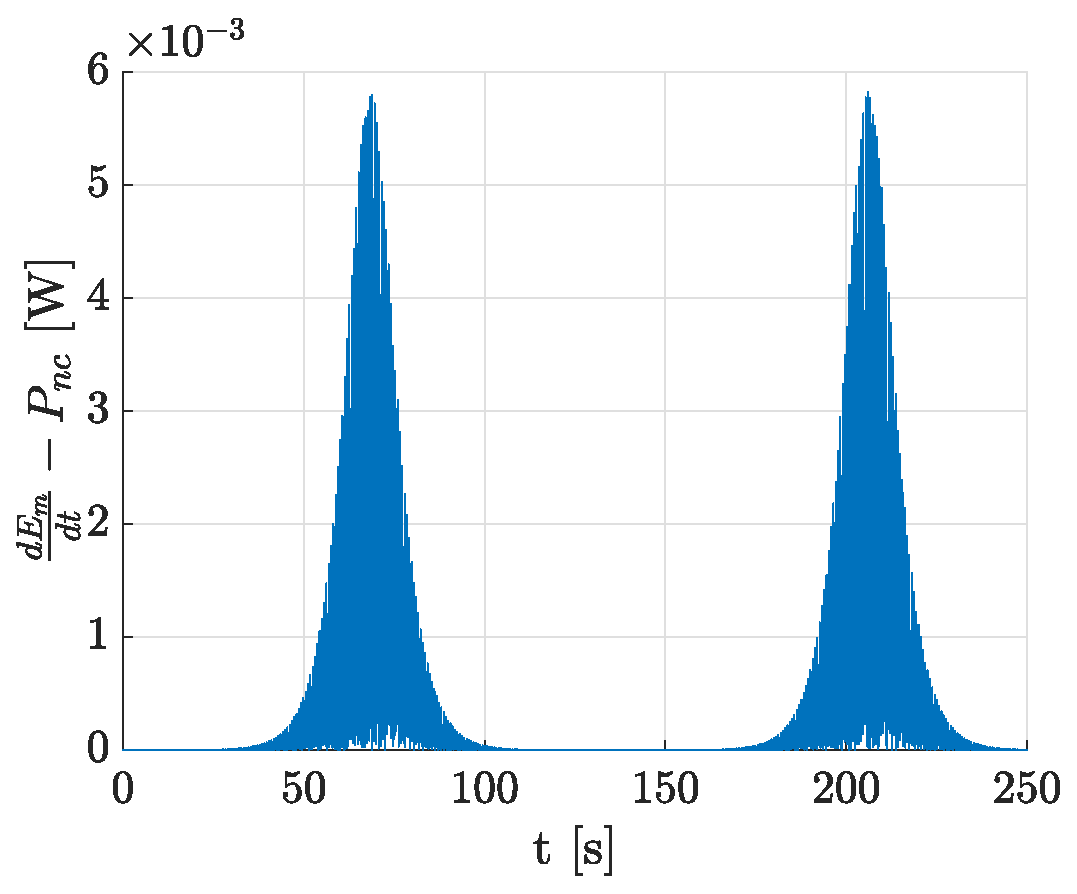
\includegraphics[width=0.55\textwidth]{graphs/c_thm.eps}
	\caption{Verification of the mechanical energy theorem by drawing the difference over time. The computations are done using a time step of $\Delta t = \SI{2d-2}{\s}$.}
	\label{fig:c-thm}
\end{figure}

%TODO : Faire une discussion sur cette figure quand le graph sera final.

\subsubsection{Varying $\Omega$}

\begin{figure}[h!]
\centering
	\begin{subfigure}[t]{0.45\textwidth}
		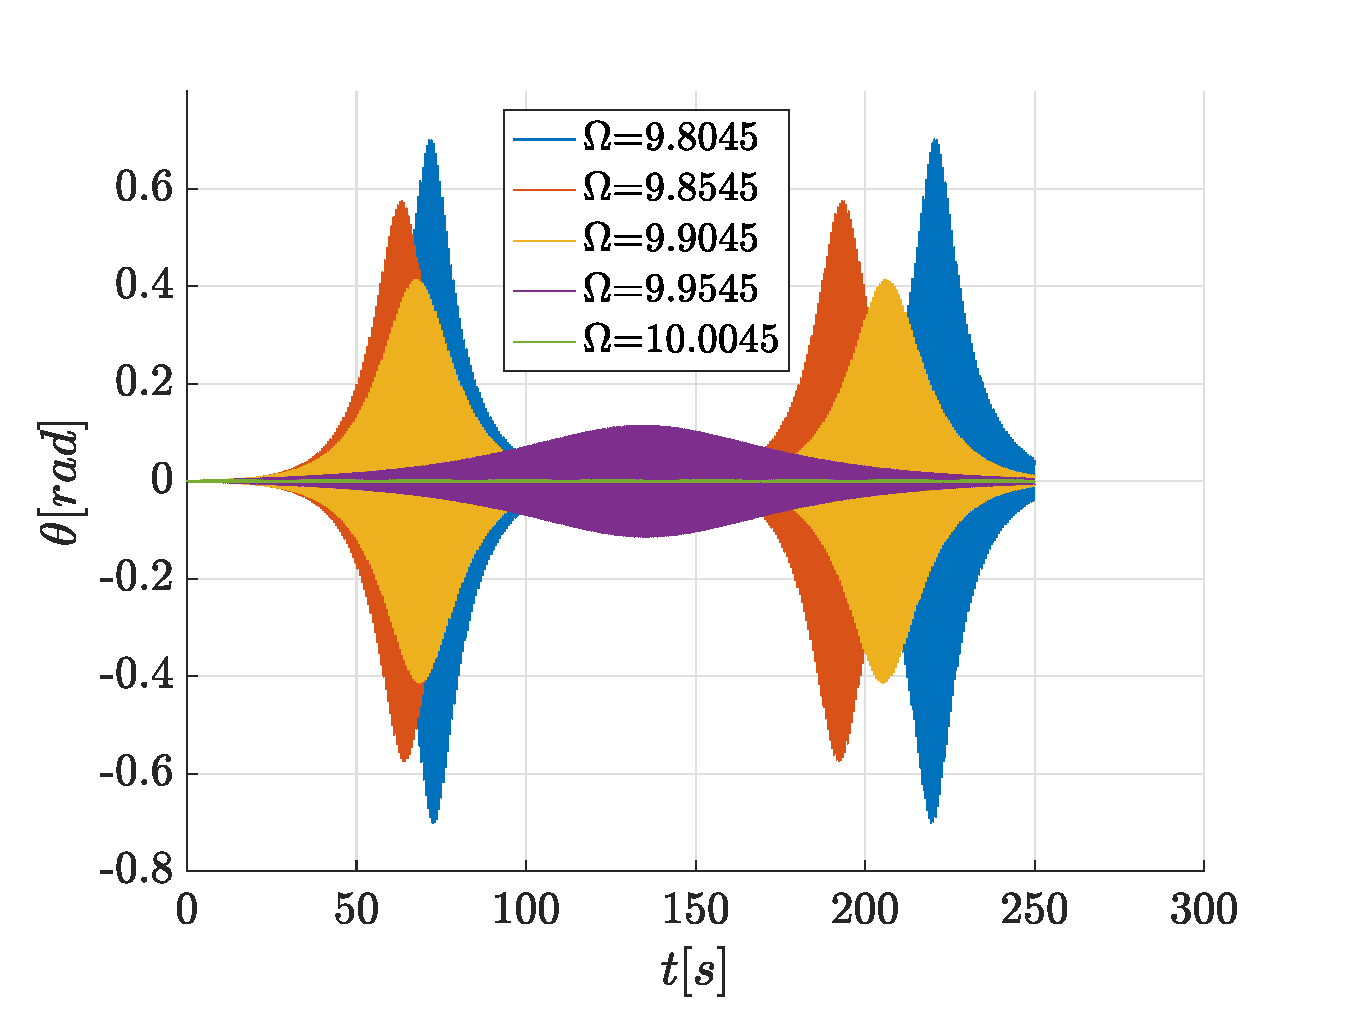
\includegraphics[width=\textwidth]{graphs/c_comptheta.eps}
		\caption{Evolution of the angle $\theta$ for 5 different $\Omega$}
		\label{fig:c-comptheta}
	\end{subfigure}
	~
	\begin{subfigure}[t]{0.45\textwidth}
		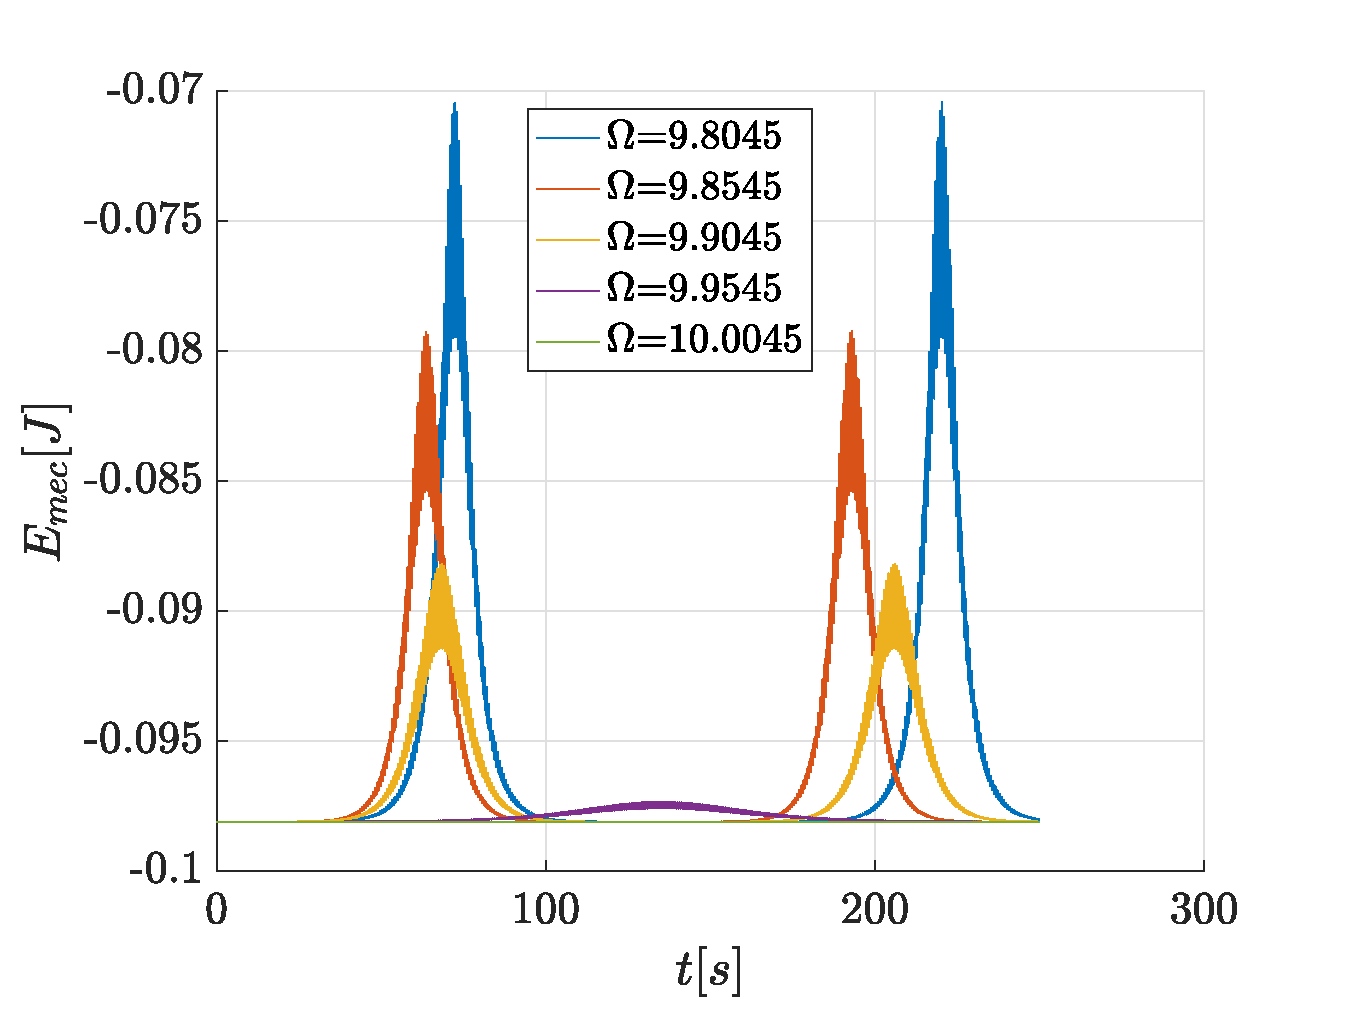
\includegraphics[width=\textwidth]{graphs/c_compemec.eps}
		\caption{Evolution of $E_m$ for 5 different $\Omega$}
		\label{fig:c-compemec}
	\end{subfigure}
	\caption{Comparison of different parameters over time for systems with different $\Omega$ around $\omega_0$}
\label{fig:c-comp}
\end{figure}

Figure \ref{fig:c-comp} was made using a time step of $\Delta t = \SI{2d-2}{\s}$, for 5 different $\Omega$ in the interval $[\omega_0-10^{-1}, \omega_0+10^{-1}]$, with the yellow plot representing the case of $\Omega = \omega_0$. A resonance phenomenon can still be observed for an excitation frequency slightly lower than $\omega_0$, as movement and energy spikes higher than that of the case of $\Omega=\omega_0$ are displayed. However, for $\Omega$ slightly higher than $\omega_0$, resonance does not occur and, for $\Omega=9.9545$ we instead observe a much weaker response, consisting of only one drawn-out spur of energy over the course of the simulation, while the system with $\Omega=10.0045$ has no visible response at this scale.

\begin{figure}[h]
\centering
	\begin{subfigure}[t]{0.45\textwidth}
		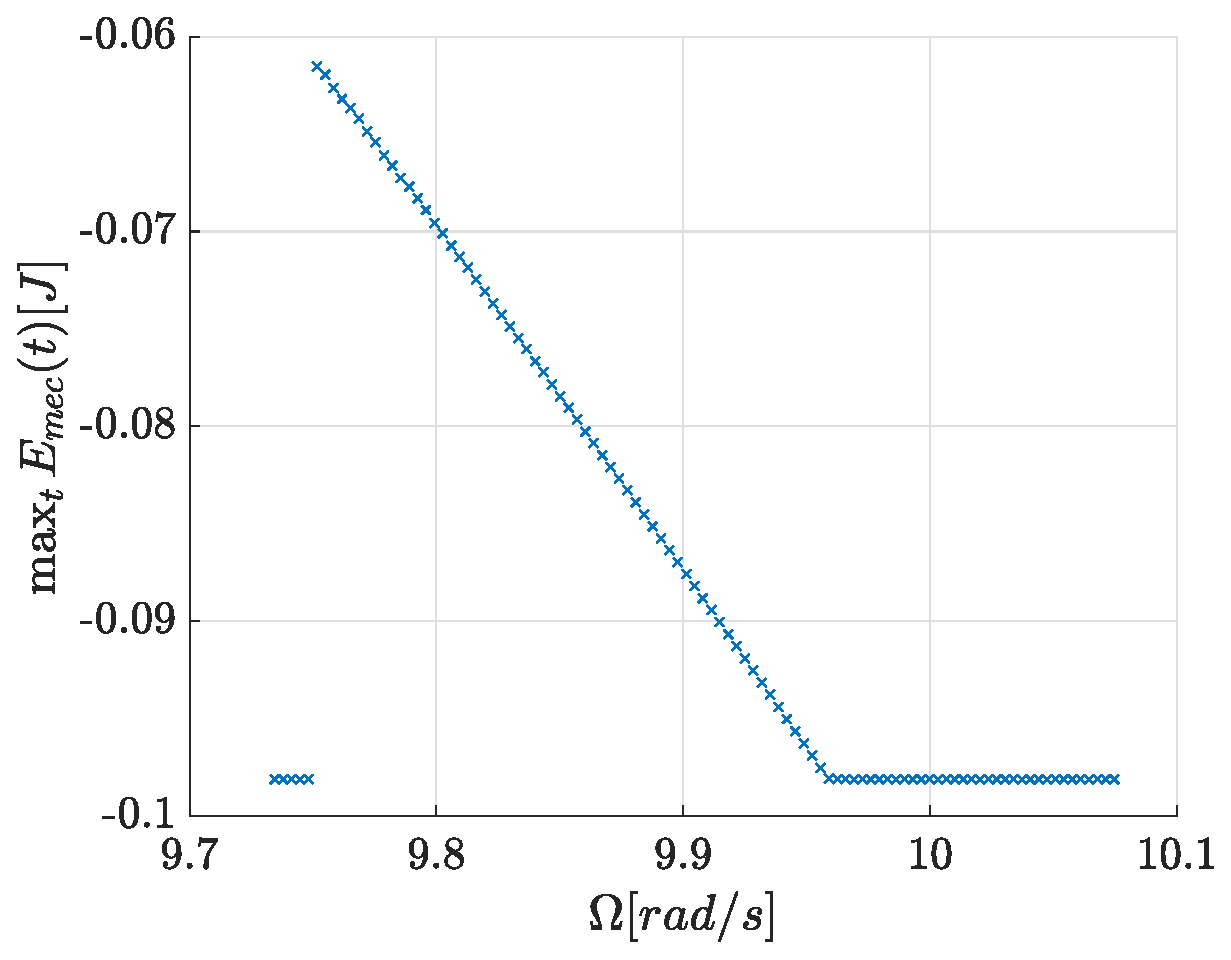
\includegraphics[width=\textwidth]{graphs/c_emax.eps}
		\caption{Maximum of mechanical energy for \num{101} simulations, using a varying $\Omega\in\left[\omega_0 - \epsilon, 2\omega_0 + \epsilon\right]$, where $\epsilon = \num{1.7d-1}$}
		\label{fig:c-emax-full}
	\end{subfigure}
	~
	\begin{subfigure}[t]{0.45\textwidth}
		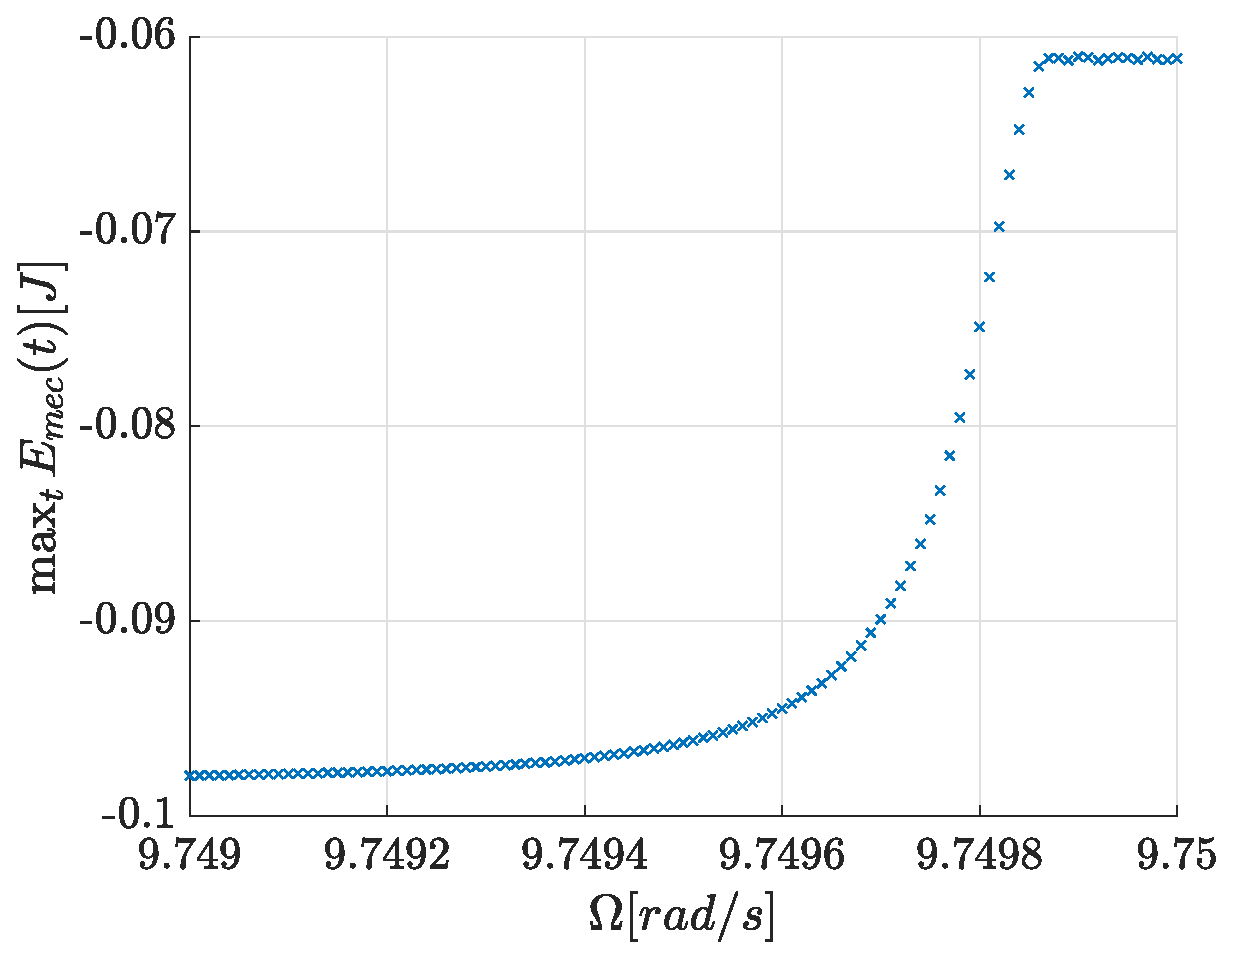
\includegraphics[width=\textwidth]{graphs/c_emaxzoom.eps}
		\caption{Zoom on the "jumping" part of \ref{fig:c-emax}. \num{101} simulations were done by varying $\Omega\in\left[9.749, 9.750 \right]$}
		\label{fig:c-emax-zoom}
	\end{subfigure}
	\caption{Maximum of mechanical energy for a varying $\Omega$ over 101 simulations}
	\label{fig:c-emax}
\end{figure}

Figure \ref{fig:c-emax} shows that the system has very little response to the excitation for $\Omega<9.749$. However the maximum of the response in energy increases exponentially until it peaks around $\Omega= 9.74985$, an excitation frequency lower than the natural frequency of the system, $\omega_0$. The maximum of the energy then decreases linearly until no response is observable from $\Omega=9.96$ onwards.

%%%%%%%%%%%%%%%%%%%%%%%%%%%%%%%%%

\subsection{Parametric excitation}

In this section, the box also moves, but this time, air resistance is considered.
The initial conditions are given by $\theta_0 = \SI{0}{\radian}$ and $\dot{\theta} = \SI{d-2}{\radian\per\second}$.
The constants are given by $\Omega = 2\omega_0$, $d = \SI{5d-3}{\m}$, $\kappa = \SI{5d-2}{\kg\per\s}$ and $t_{end} = \SI{100}{\s}$.

\subsubsection{Verification of the mechanical energy theorem}\label{sec:d-thm}

The method here is the same described in section \ref{sec:c-thm}, and the result can be seen on figure \ref{fig:d-thm}.

\begin{figure}[h]
\centering
\begin{subfigure}[t]{0.45\textwidth}
	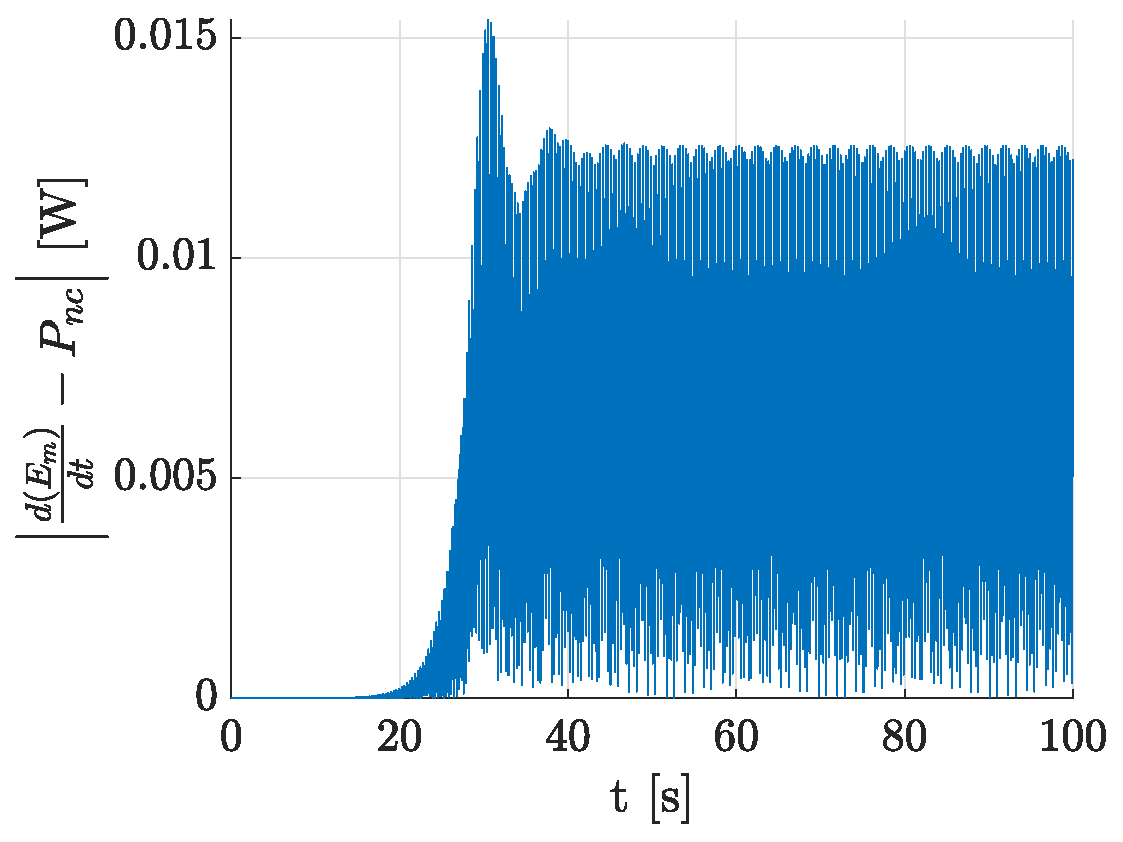
\includegraphics[width=\textwidth]{graphs/d_thm.eps}
	\caption{Difference of the derivative of mechanical energy with the power of non-conservative forces}
	\label{fig:d-thm-energie}
\end{subfigure}
~
\begin{subfigure}[t]{0.45\textwidth}
	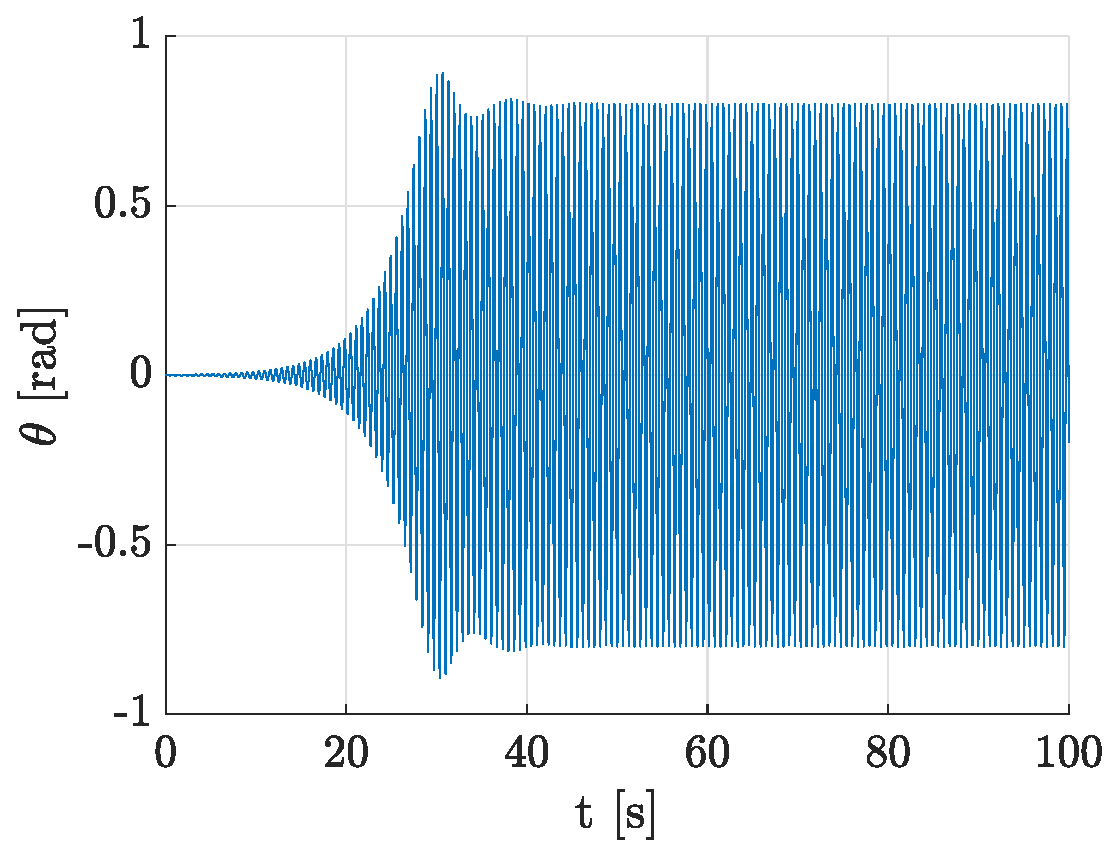
\includegraphics[width=\textwidth]{graphs/d_theta.eps}
	\caption{Angle $\theta$ of the pendulum over time}
	\label{fig:d-thm-theta}
\end{subfigure}
\caption{Simulation describing the conservation of energy. The time step is $\Delta t=\SI{2d-2}{\s}$, which implies that the simulation was done over \num{5000} steps}
\label{fig:d-thm}
\end{figure}

Figure \ref{fig:d-thm} is the verification of the mechanical energy theorem, where the derivative of $E_{mec}$ has been computed numerically.
The theorem is more or less verified in the \num{20} first seconds of the simulation.
This can be observed on figure \ref{fig:d-thm-energie} where the curve is close to 0.
After that, the difference changes drastically and oscillates with a great amplitude, which seems to implies that the theorem is not verified after \SI{20}{\s}.
Figure \ref{fig:d-thm-theta} shows the evolution of $\theta$ over time.
Before \SI{20}{\s}, the oscillations are considered as small.
But after that, the oscillation's amplitude grows exponentially with much bigger oscillations, until ~\SI{30}{\s}.
At this time, its maximum is reached and it stabilizes its oscillation.\\

Numerical methods are not as perfect as an analytical solution, and it is the reason why the theorem is not verified numerically after \SI{20}{\s}.
When the pendulum does small oscillations (before \SI{20}{\s}), the mechanical energy does not vary a lot.
Thus, the derivative, which measures the changes in the mechanical energy, is close to the analytical solution, and it is the reason why the curve is so close to 0.
After that, the pendulum oscillates with a great amplitude, which implies a big variation of the mechanical energy, and this is the reason why the difference as great as it is.
The error becomes great because the numerical method is not good enough with big variations.
To decrease this error, it is possible to reduce $\Delta t$ for the same simulation.
It will reduce the amplitude of the variation between two computations, thus increasing the precision of the derivative of the mechanical energy.
This is the reason why, on figure \ref{fig:d-thm-energie}, the theorem does not seem to be verified although the theorem is proven analytically.\\

The behaviour of the pendulum over time can be explained by two factors.
First, it the oscillation of the box.
At the beginning, the box and the pendulum are not synced, because the initial conditions are different.
But progressively, the pendulum gains amplitude until ~\SI{30}{\s}, where the pendulum and the box are synced together, and after that point, both remains synced which is the reason why the pendulum is so stable after a moment.
The second factor is the air resistance.
This force depends on the speed and a coefficient.
The drastic increase of the amplitude of $\theta$ also increases the angular speed of the pendulum.
Thus, the air resistance follows and greatly increases too.
It impacts the stabilization of oscillation of the pendulum and is the reason why it does not keep the amplitude measured at \SI{30}{\s}.
When exceeding the stable amplitude, air resistance is too big compared to the other force, and restrains the pendulum's amplitude.
Thus, it stabilizes.\\
%TODO : Est-ce que ce dernier paragraphe est pertinent ?

\subsubsection{Varying $\Omega$}
In this section, $\Omega$ varies around a $2\omega_0$, and the maximum of mechanical energy is observed with respect to $\Omega$.

Figure \ref{fig:d-emax} shows the maximum mechanical energy for a range of $\Omega$.
A resonance phenomenon can be observed on figures \ref{fig:d-emax-full}, around $\Omega=\SI{19.15}{\radian\per\s}$.
Figure \ref{fig:d-emax-close} shows a closer look on the curve around this condition.
It can be seen that the maximum reached by the mechanical energy increases drastically, until a point where it just slowly decreases.

\begin{figure}[h]
\centering
	\begin{subfigure}[t]{0.45\textwidth}
		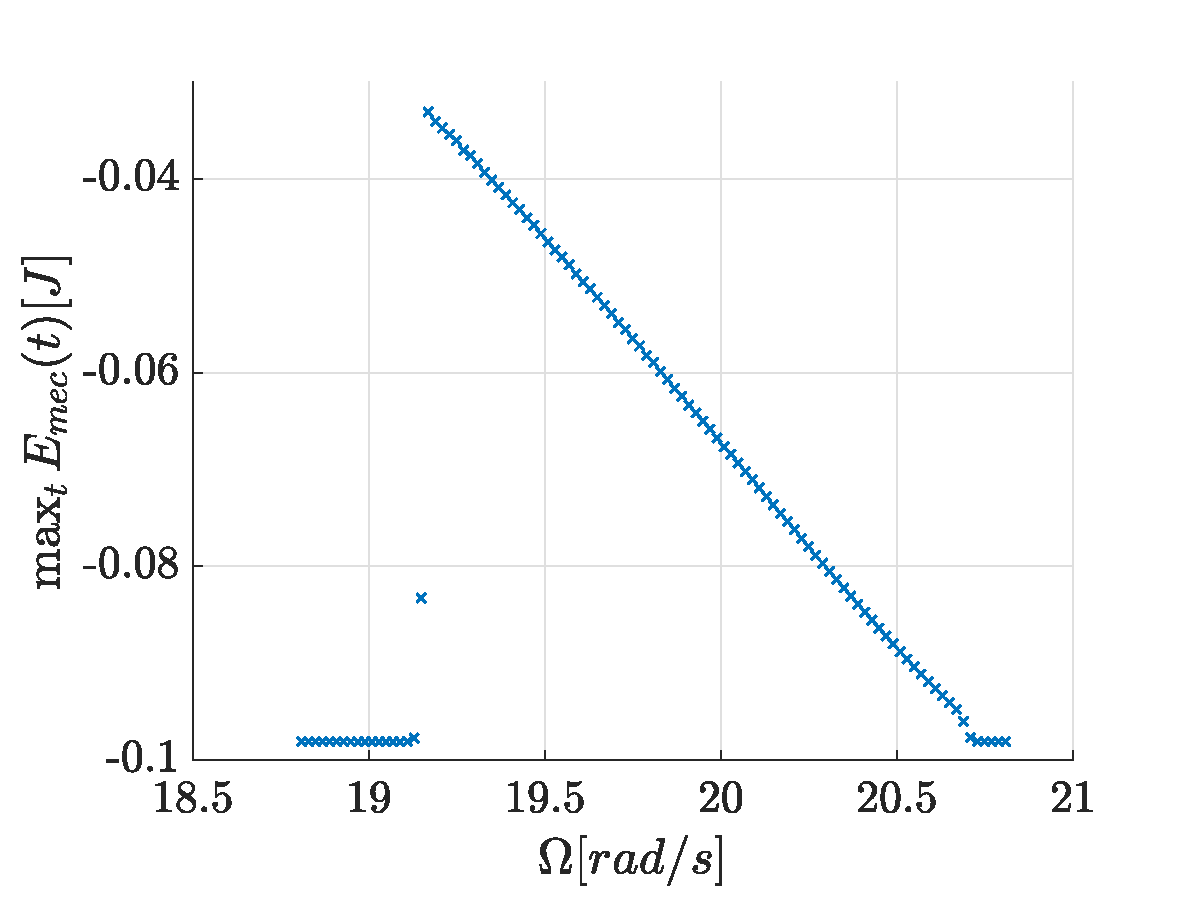
\includegraphics[width=\textwidth]{graphs/d_emax_full.eps}
		\caption{Maximum of mechanical energy, using a varying $\Omega\in\left[2\omega_0 - \epsilon, 2\omega_0 + \epsilon\right]$, where $\epsilon = \num{1}$.}
		\label{fig:d-emax-full}
	\end{subfigure}
	~
	\begin{subfigure}[t]{0.45\textwidth}
		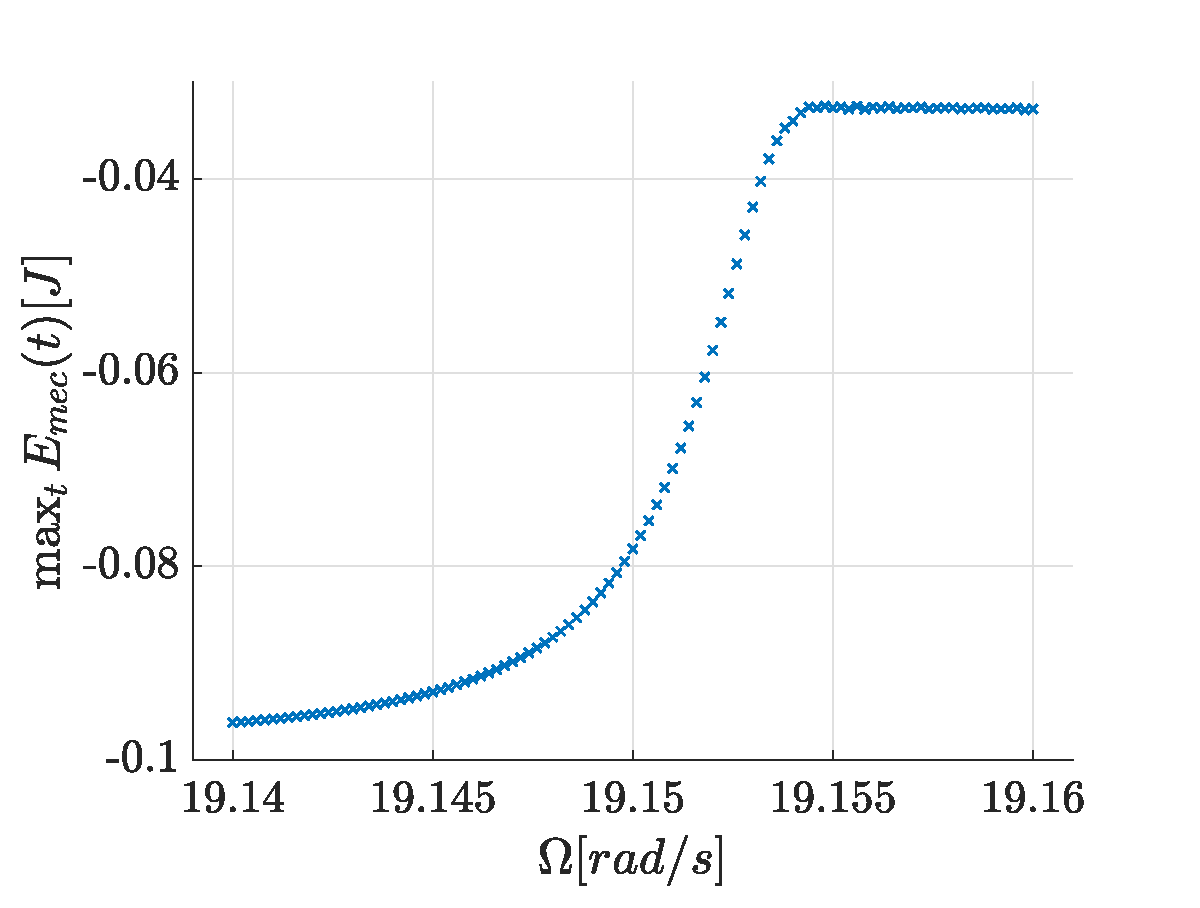
\includegraphics[width=\textwidth]{graphs/d_emax_close.eps}
		\caption{Zoom on the "jumping" part of \ref{fig:d-emax-full}. $\Omega$ varies on a smaller range: $\Omega\in\left[\num{19.15} - \epsilon, \num{19.15} + \epsilon\right]$, where $\epsilon = \num{1d-2}$.}
		\label{fig:d-emax-close}
	\end{subfigure}
	\caption{Maximum of mechanical energy for a varying $\Omega$ over 101 simulations}
	\label{fig:d-emax}
\end{figure}

This can be observed in figure \ref{fig:d-comp}.
On figure \ref{fig:d-comp-theta}, for $\Omega=\SI{18.8091}{\radian\per\s}$ and $\Omega=\SI{20.8091}{\radian\per\s}$, it can be observed no respond of the pendulum to the box's excitation, which also means a low maximum mechanical energy for both of them, as seen on figure \ref{fig:d-comp-emec}.
However, between these values, the others reacts to the excitation.
All of the remaining points are located in the decreasing line of figure \ref{fig:d-emax-full}, and it can be seen the reason why the mechanical decreases with $\Omega$ increasing after the resonance: the maximum amplitude of $\theta$ decreases.
This comes from the resonance phenomenon, which changes the maximum amplitude of the pendulum with respect to $\Omega$.\\

\begin{figure}[h]
\centering
	\begin{subfigure}[t]{0.45\textwidth}
		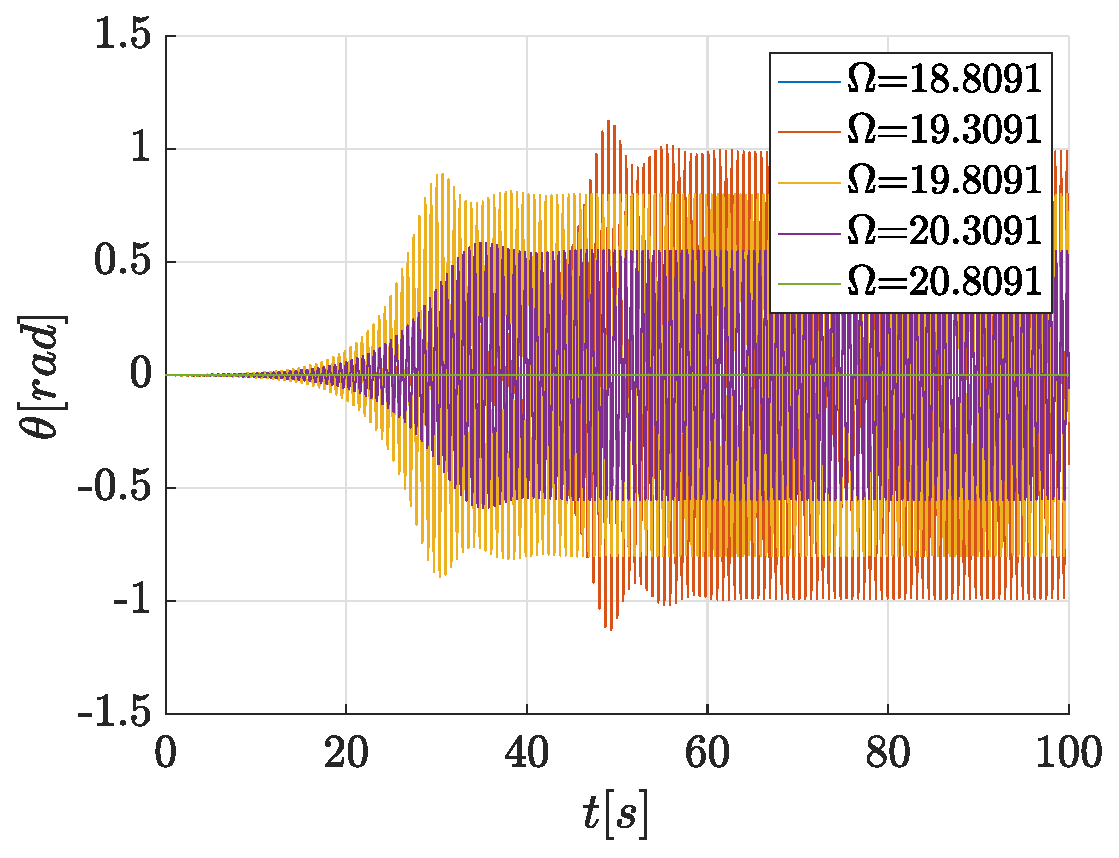
\includegraphics[width=\textwidth]{graphs/d_comptheta.eps}
		\caption{Evolution of the angle $\theta$ for 5 different $\Omega$}
		\label{fig:d-comp-theta}
	\end{subfigure}
	~
	\begin{subfigure}[t]{0.45\textwidth}
		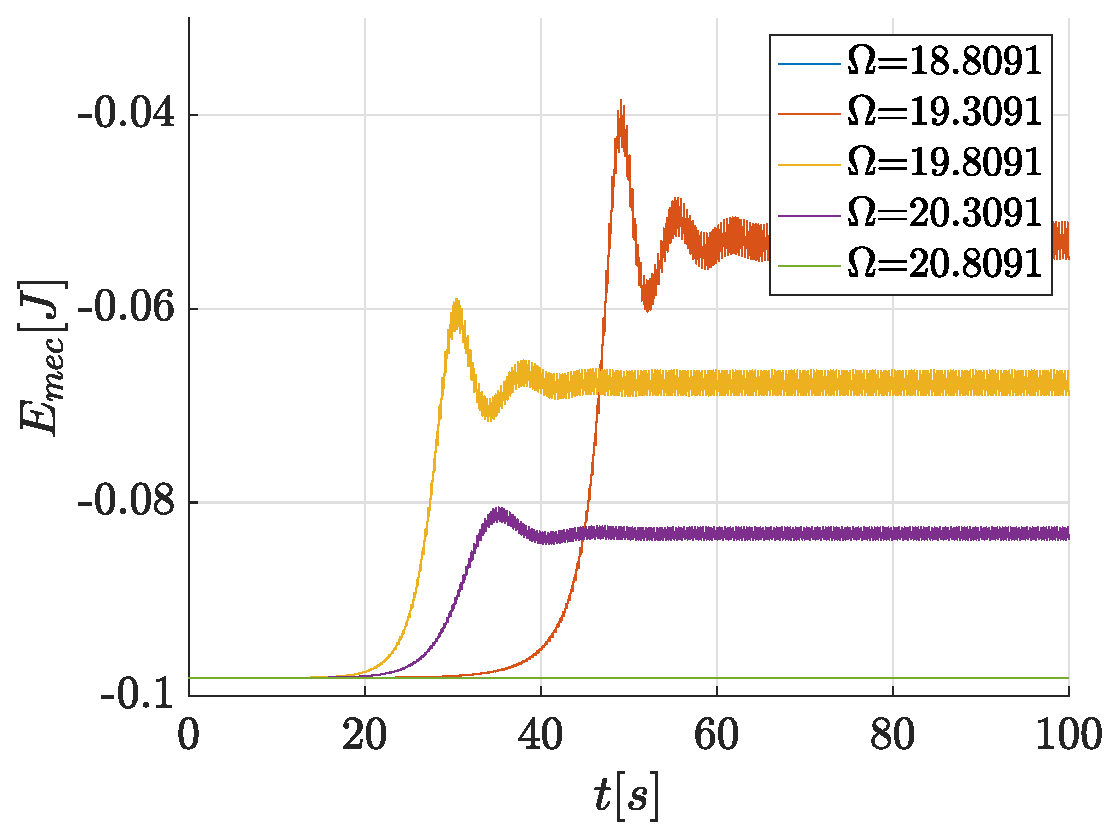
\includegraphics[width=\textwidth]{graphs/d_compemec.eps}
		\caption{Evolution of the mechanical energy $E_{mec}$ for 5 different $\Omega$}
		\label{fig:d-comp-emec}
	\end{subfigure}
	\caption{Comparison of different parameters over time for systems with different $\Omega$ around $\omega_0$}
	\label{fig:d-comp}
\end{figure}

The evolution of the pendulum over time with respect to $\Omega=2\omega_0$, as discussed in section \ref{sec:d-thm}, also applies here.

%%%%%%%%%%%%%%%%%%%%%%%%%%%%%%%%%

\subsection{Poincaré section: chaos without air resistance}
This section will focus on chaotic movements of the pendulum, by neglecting air resistance.
The constants are given by $\Omega = \omega_0$, $d=\SI{4d-2}{\m}$ and $\kappa=\SI{0}{\kg\per\s}$.

\subsubsection{Convergence study on the final angle $\theta$}
First, a convergence study of the final angle is done.
The initial conditions are given by $\theta_0=\SI{0}{\radian}$ and $\dot{\theta_0}=\SI{d-2}{\radian\per\second}$.
The duration of the simulation is given by $t_\text{end} = 20\times\frac{2\pi}{\Omega} \approx \SI{12.69}{\s}$.
The resulting convergence study is given by figure \ref{fig:e-conv}.

\begin{figure}[h]
	\centering
	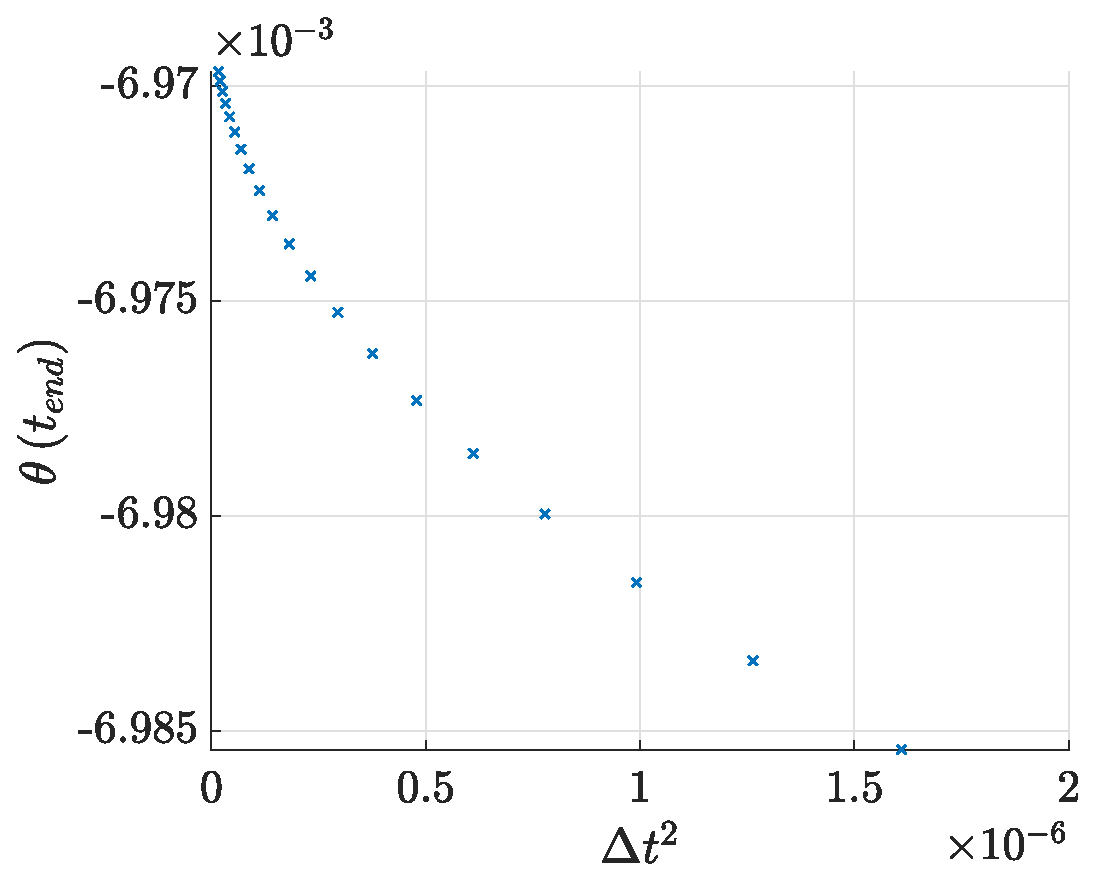
\includegraphics[width=0.6\textwidth]{graphs/e_conv.eps}
	\caption{Convergence study on the final angle over \num{100} simulations} %TODO : C'est censé être une droite ! Je fais quoi avec ça ?
	\label{fig:e-conv}
\end{figure}

%TODO : Analyser ce graph.

\subsubsection{Poincaré sections}
This section focuses on the drawing of some poincaré section, using different initial conditions.
All of them results in figure \ref{fig:e-pc}.

\begin{figure}[h]
\centering
	\begin{subfigure}[t]{0.45\textwidth}
		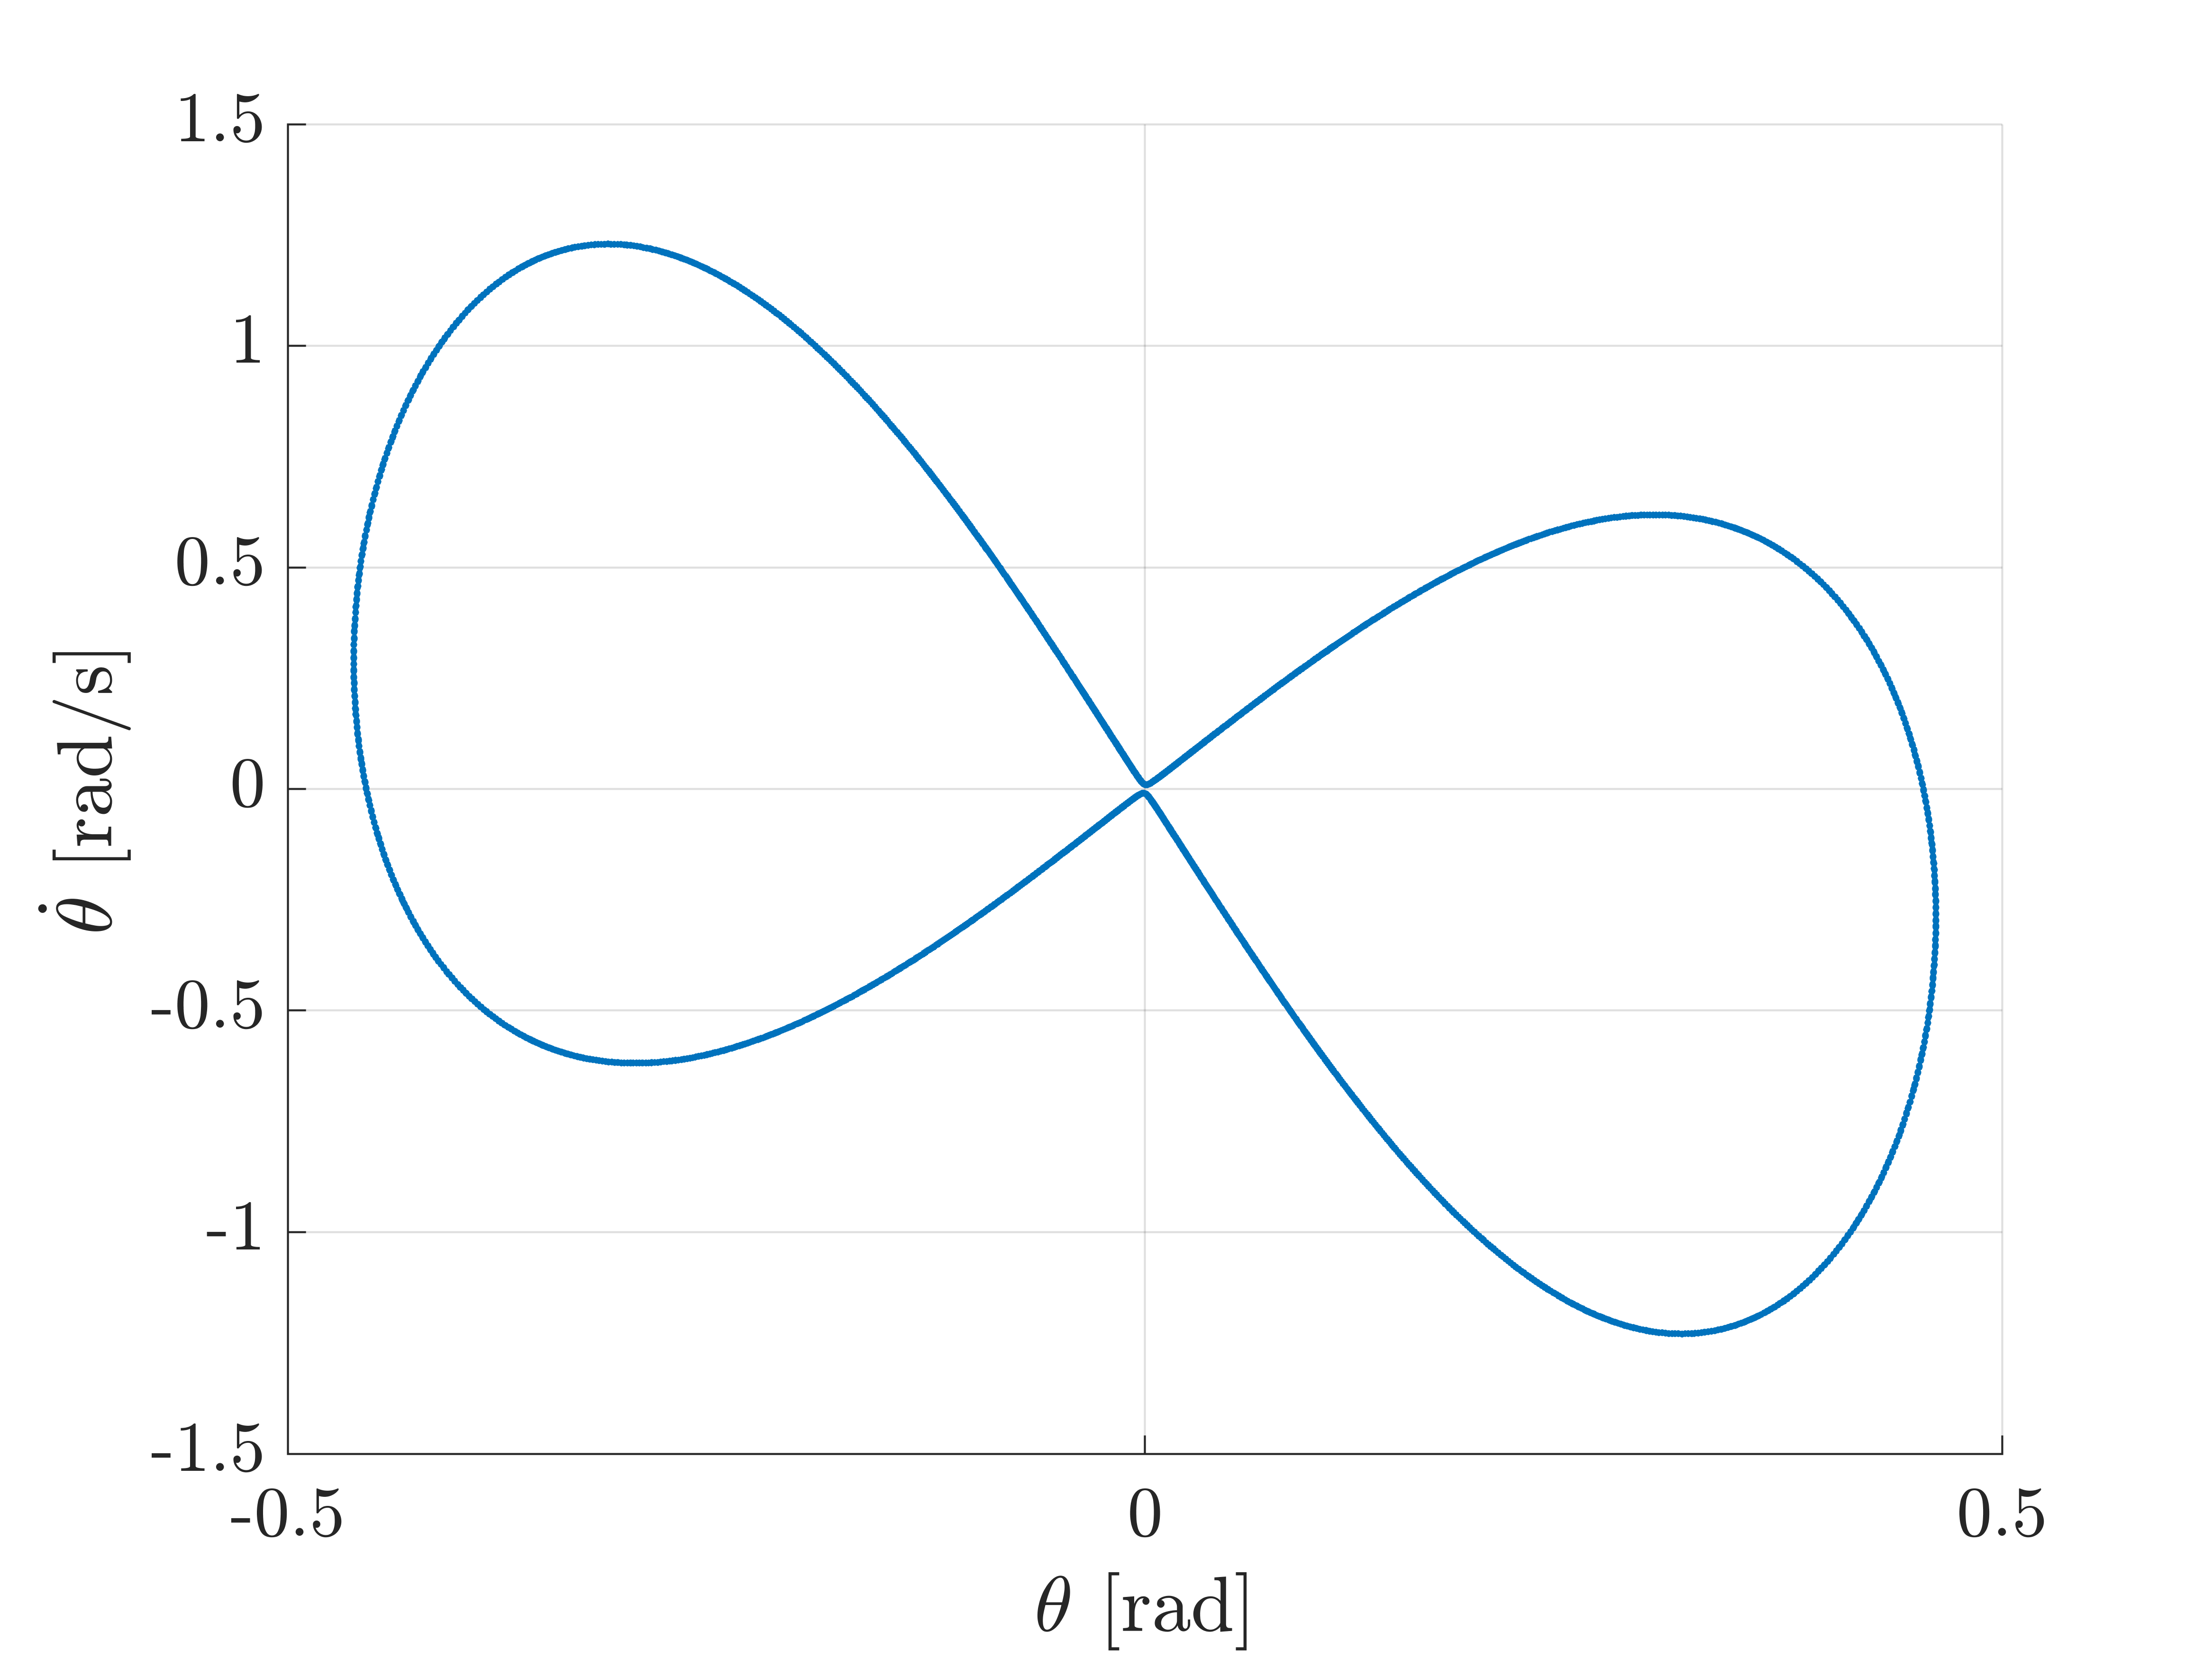
\includegraphics[width=\textwidth]{graphs/e_poincare_MK8.png}
		\caption{Non-chaotic simulation of initial conditions: $\theta_0 = \SI{0}{\radian}$ and $\dot{\theta_0}=\SI{1d-2}{\radian\per\s}$.}
		\label{fig:e-pc-MK8}
	\end{subfigure}
	~
	\begin{subfigure}[t]{0.45\textwidth}
		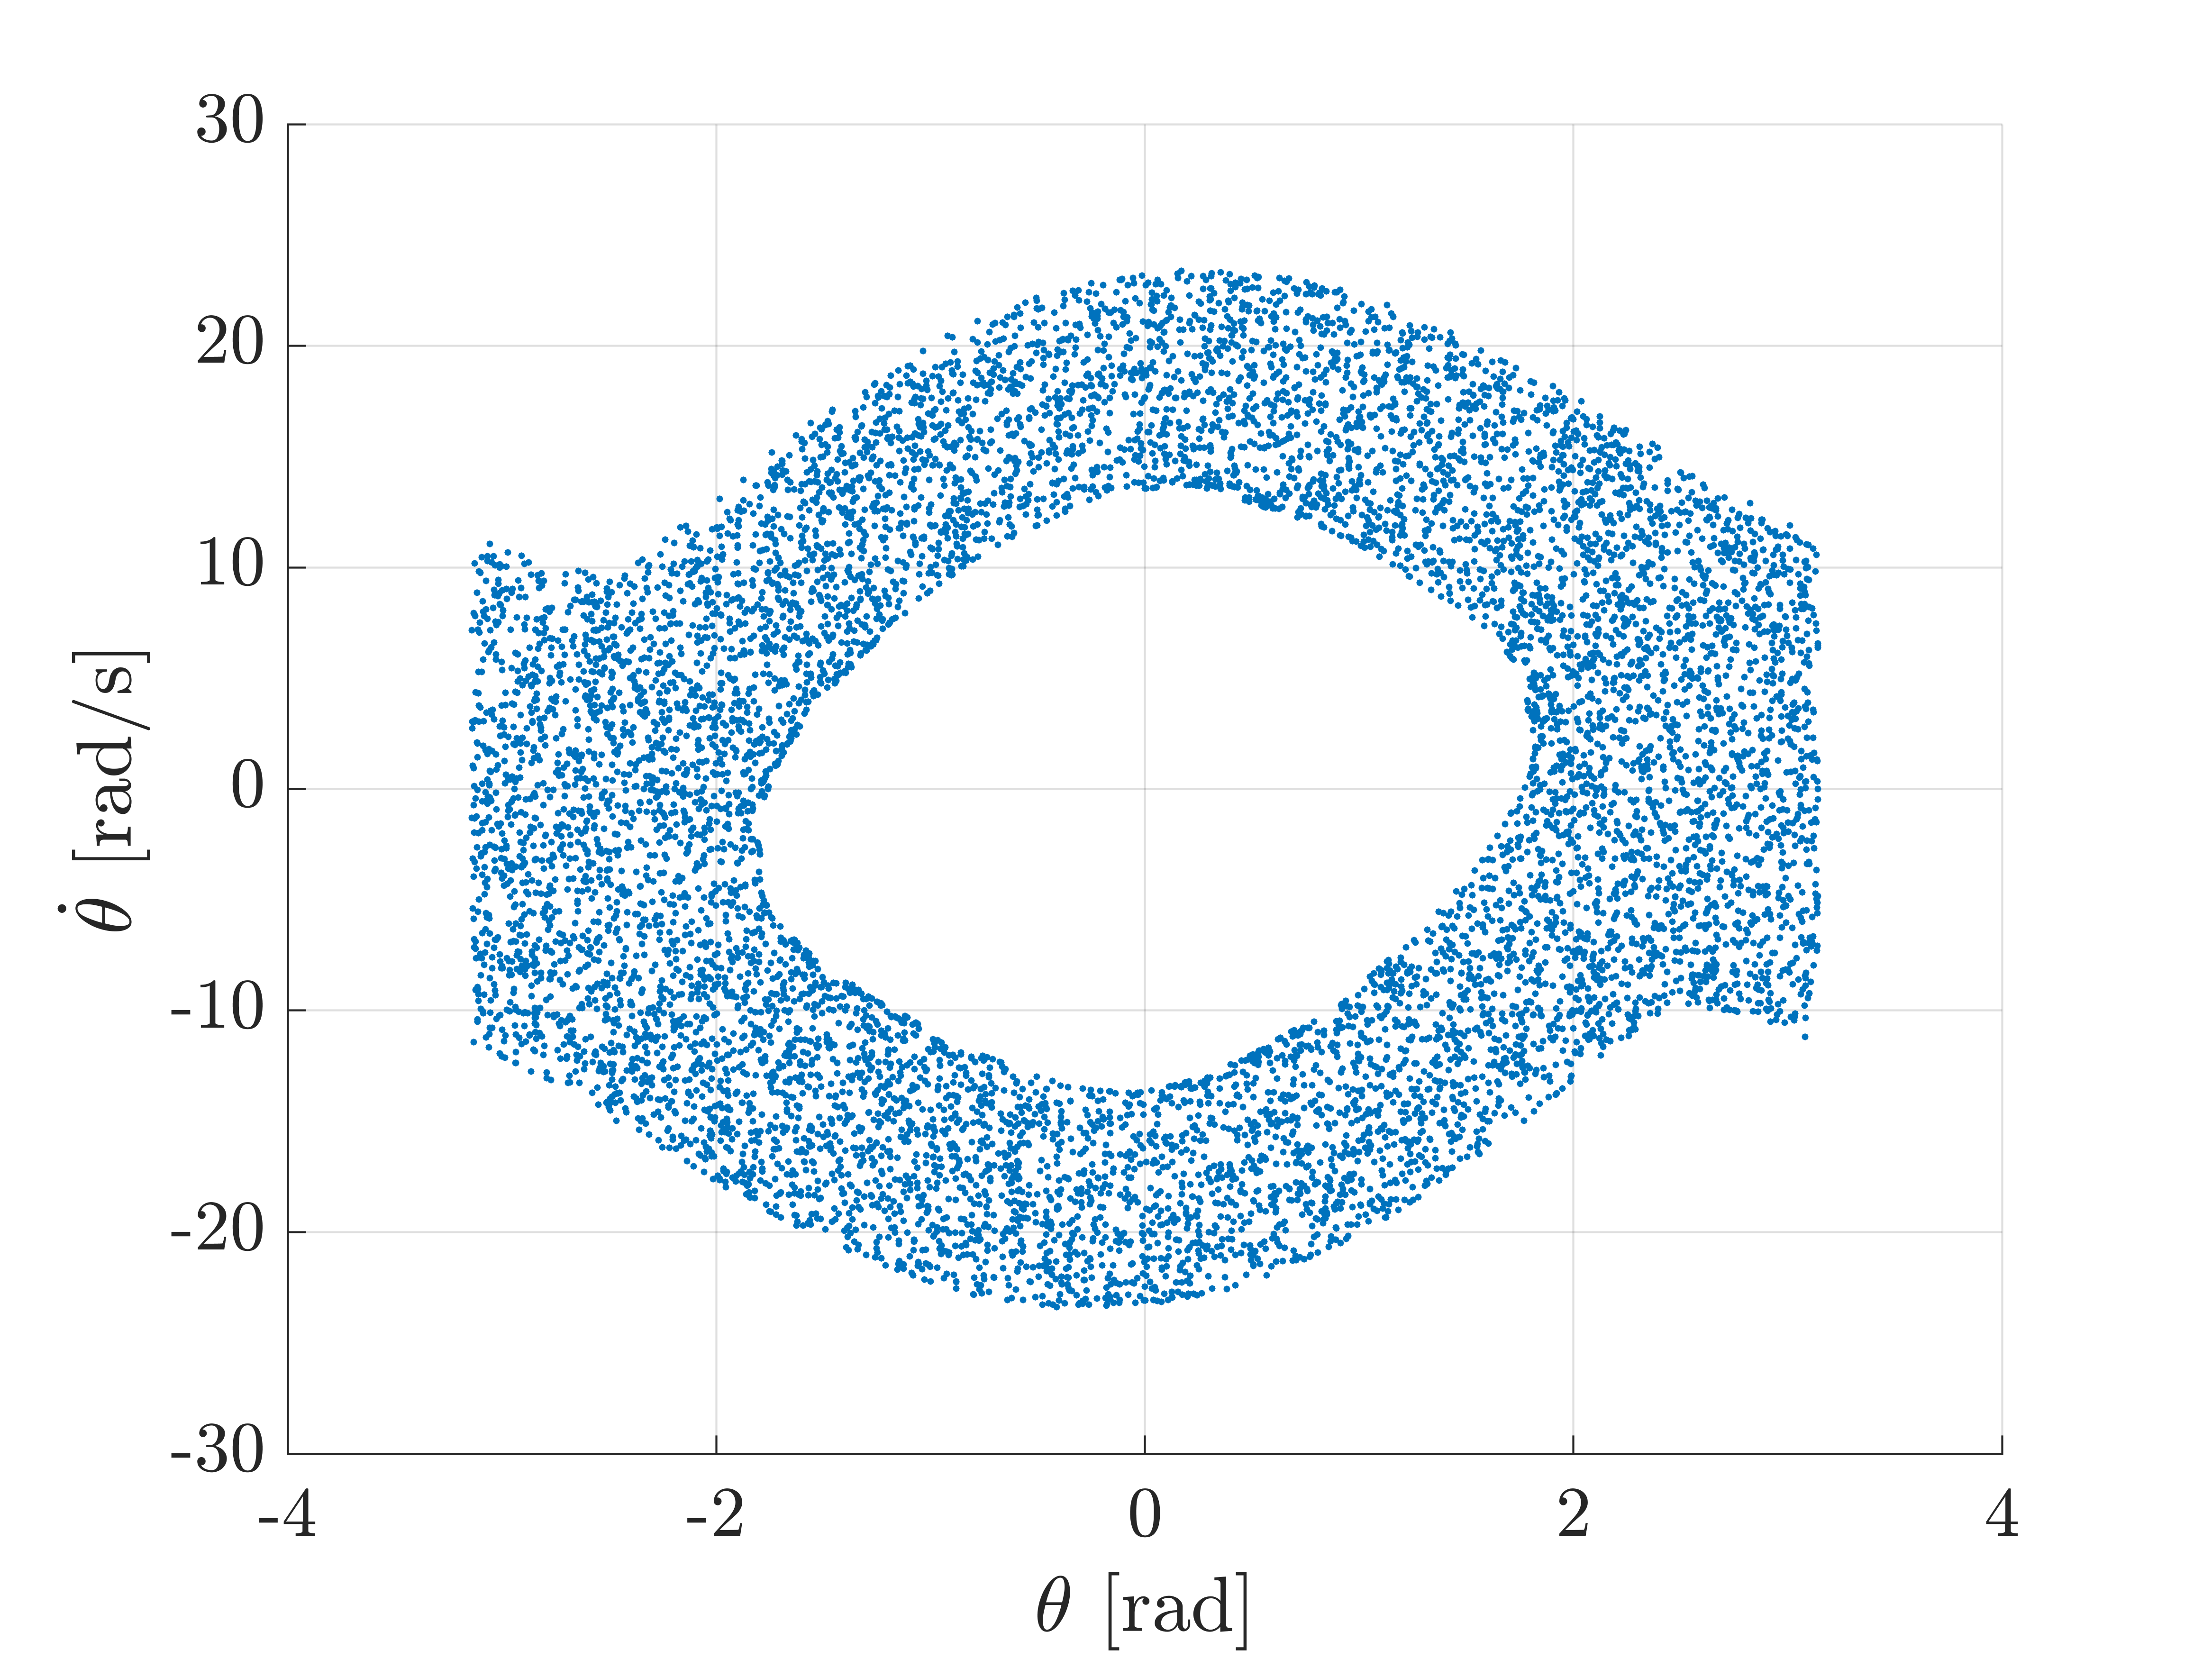
\includegraphics[width=\textwidth]{graphs/e_poincare_chaos1.png}
		\caption{Chaotic simulation of initial conditions: $\theta_0 = \SI{\pi}{\radian}$ and $\dot{\theta_0}=\SI{1d-2}{\radian\per\s}$.}
		\label{fig:e-pc-chaos1}
	\end{subfigure}
	\newline
	\begin{subfigure}[t]{0.45\textwidth}
		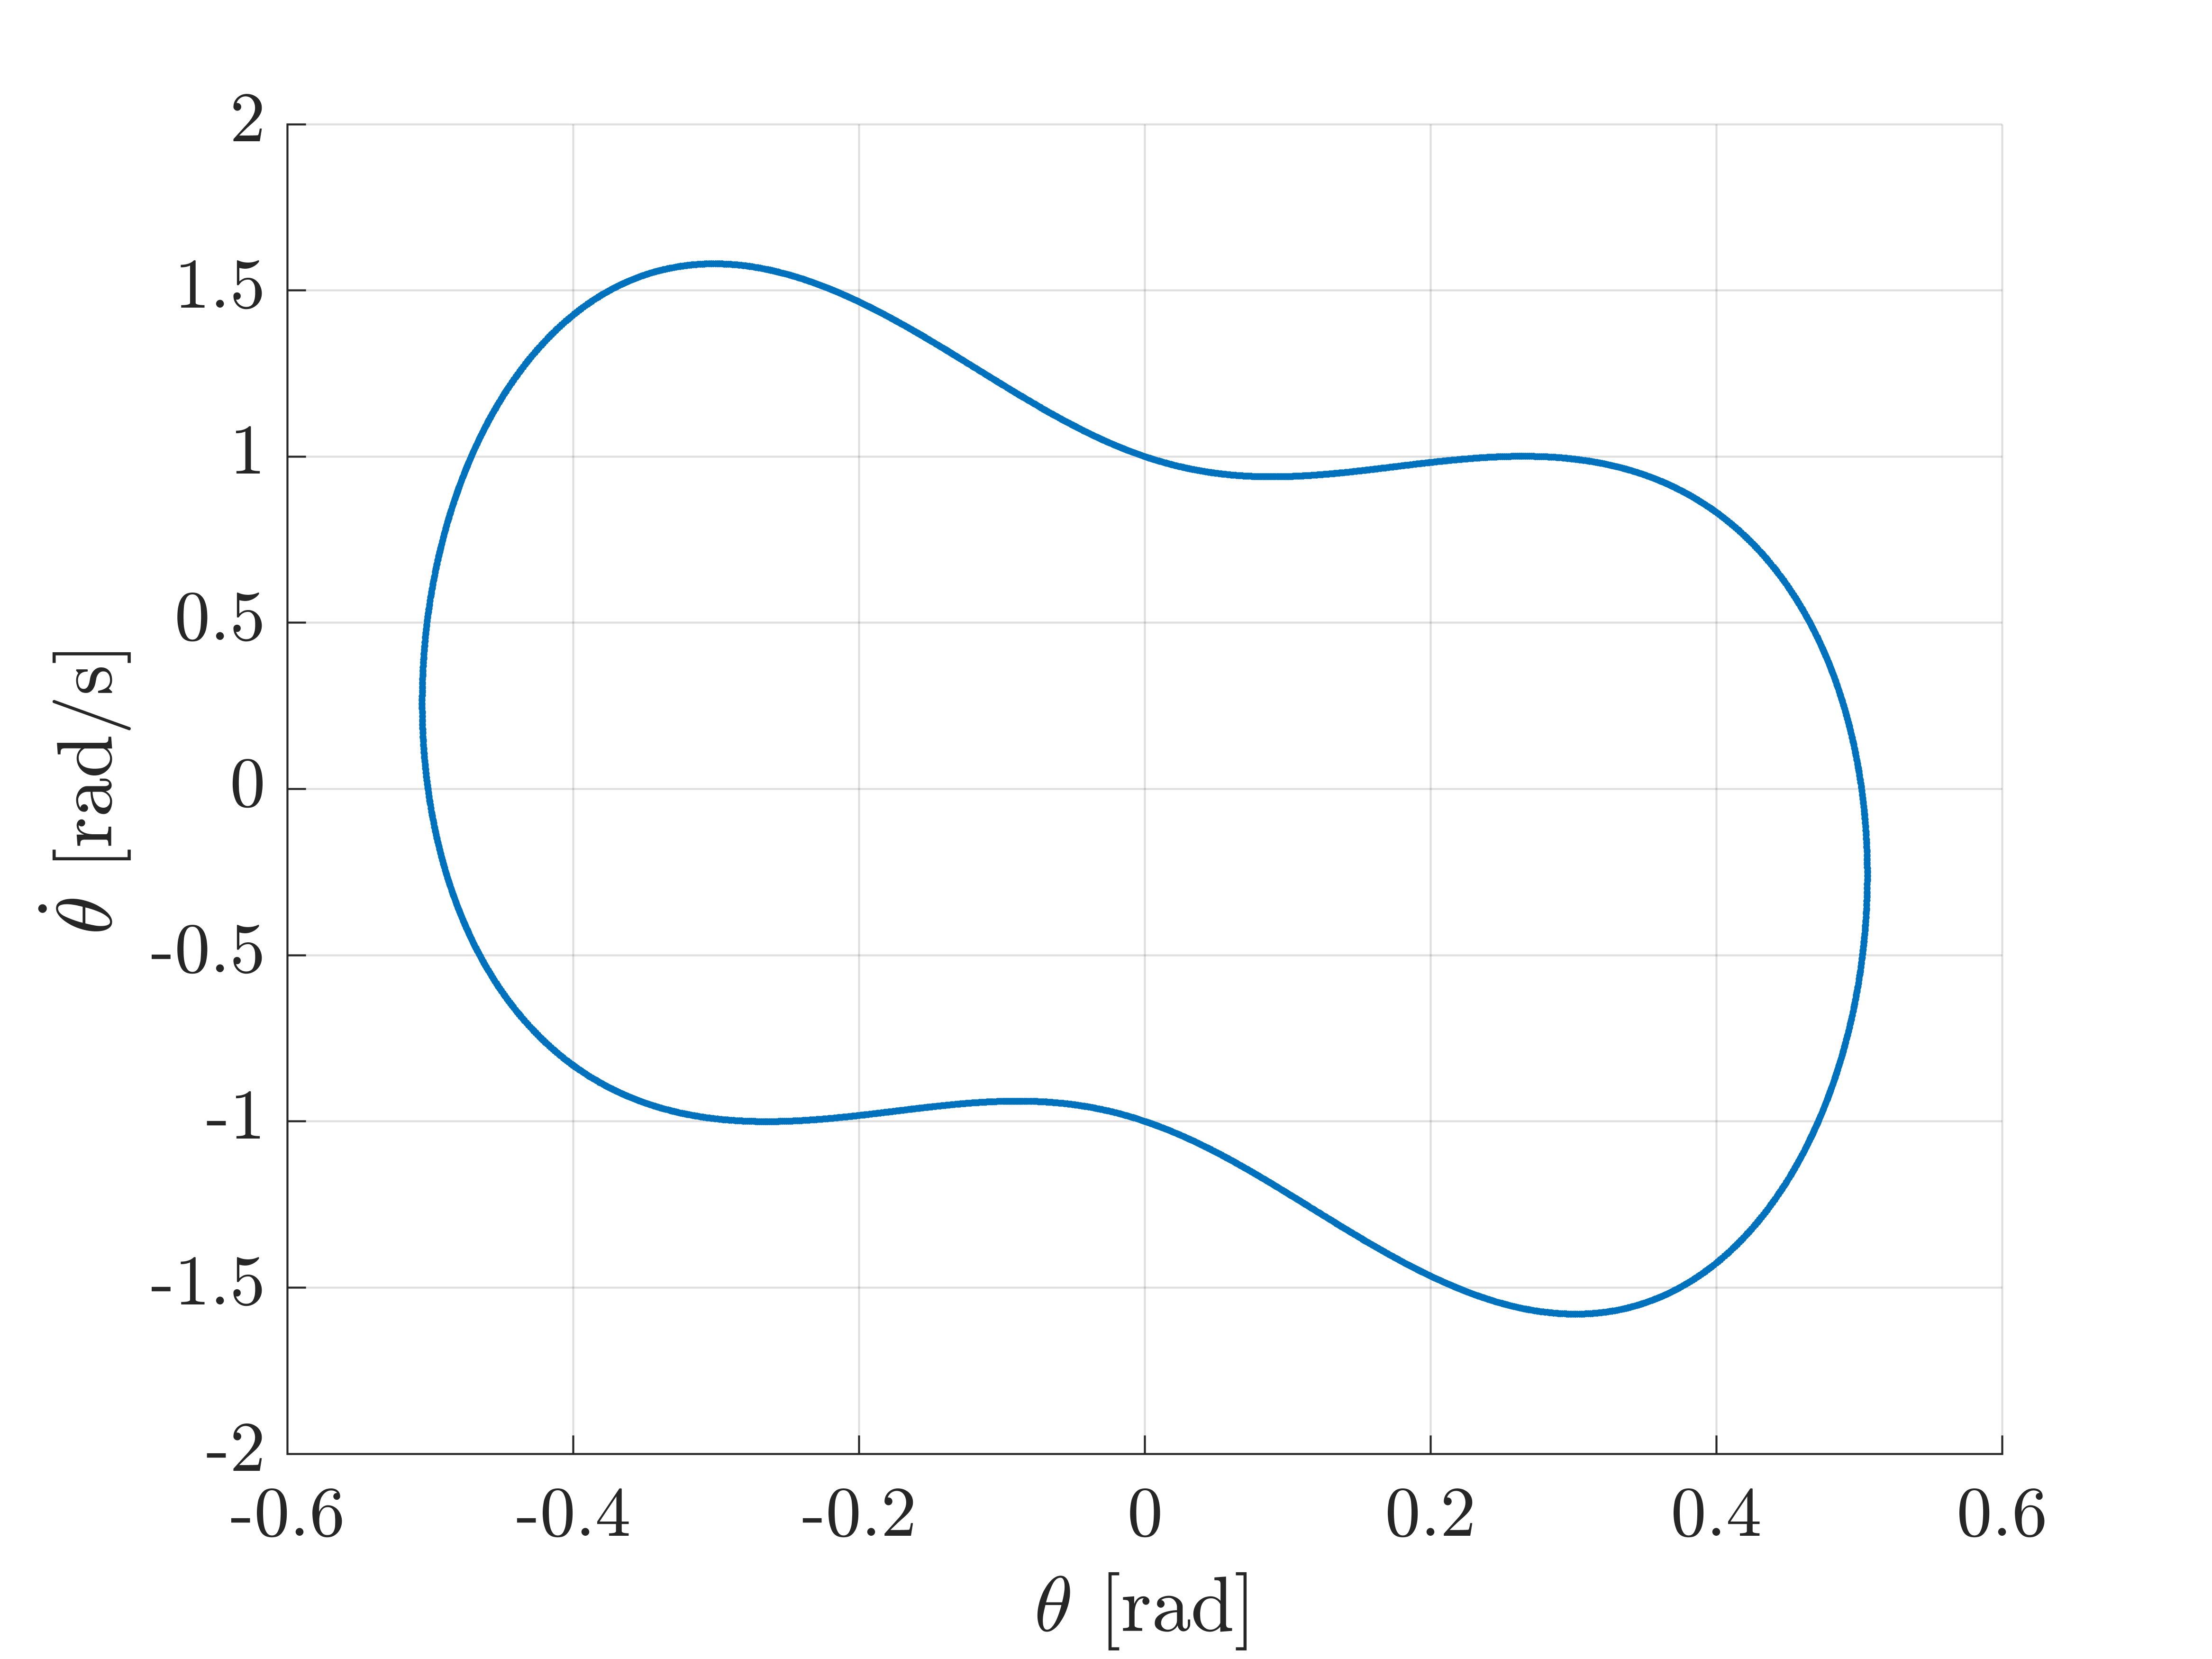
\includegraphics[width=\textwidth]{graphs/e_poincare_peanut.png}
		\caption{Non-chaotic simulation of initial conditions: $\theta_0 = \SI{1e-6}{\radian}$ and $\dot{\theta_0}=\SI{1}{\radian\per\s}$.}
		\label{fig:e-pc-peanut}
	\end{subfigure}
	~
	\begin{subfigure}[t]{0.45\textwidth}
		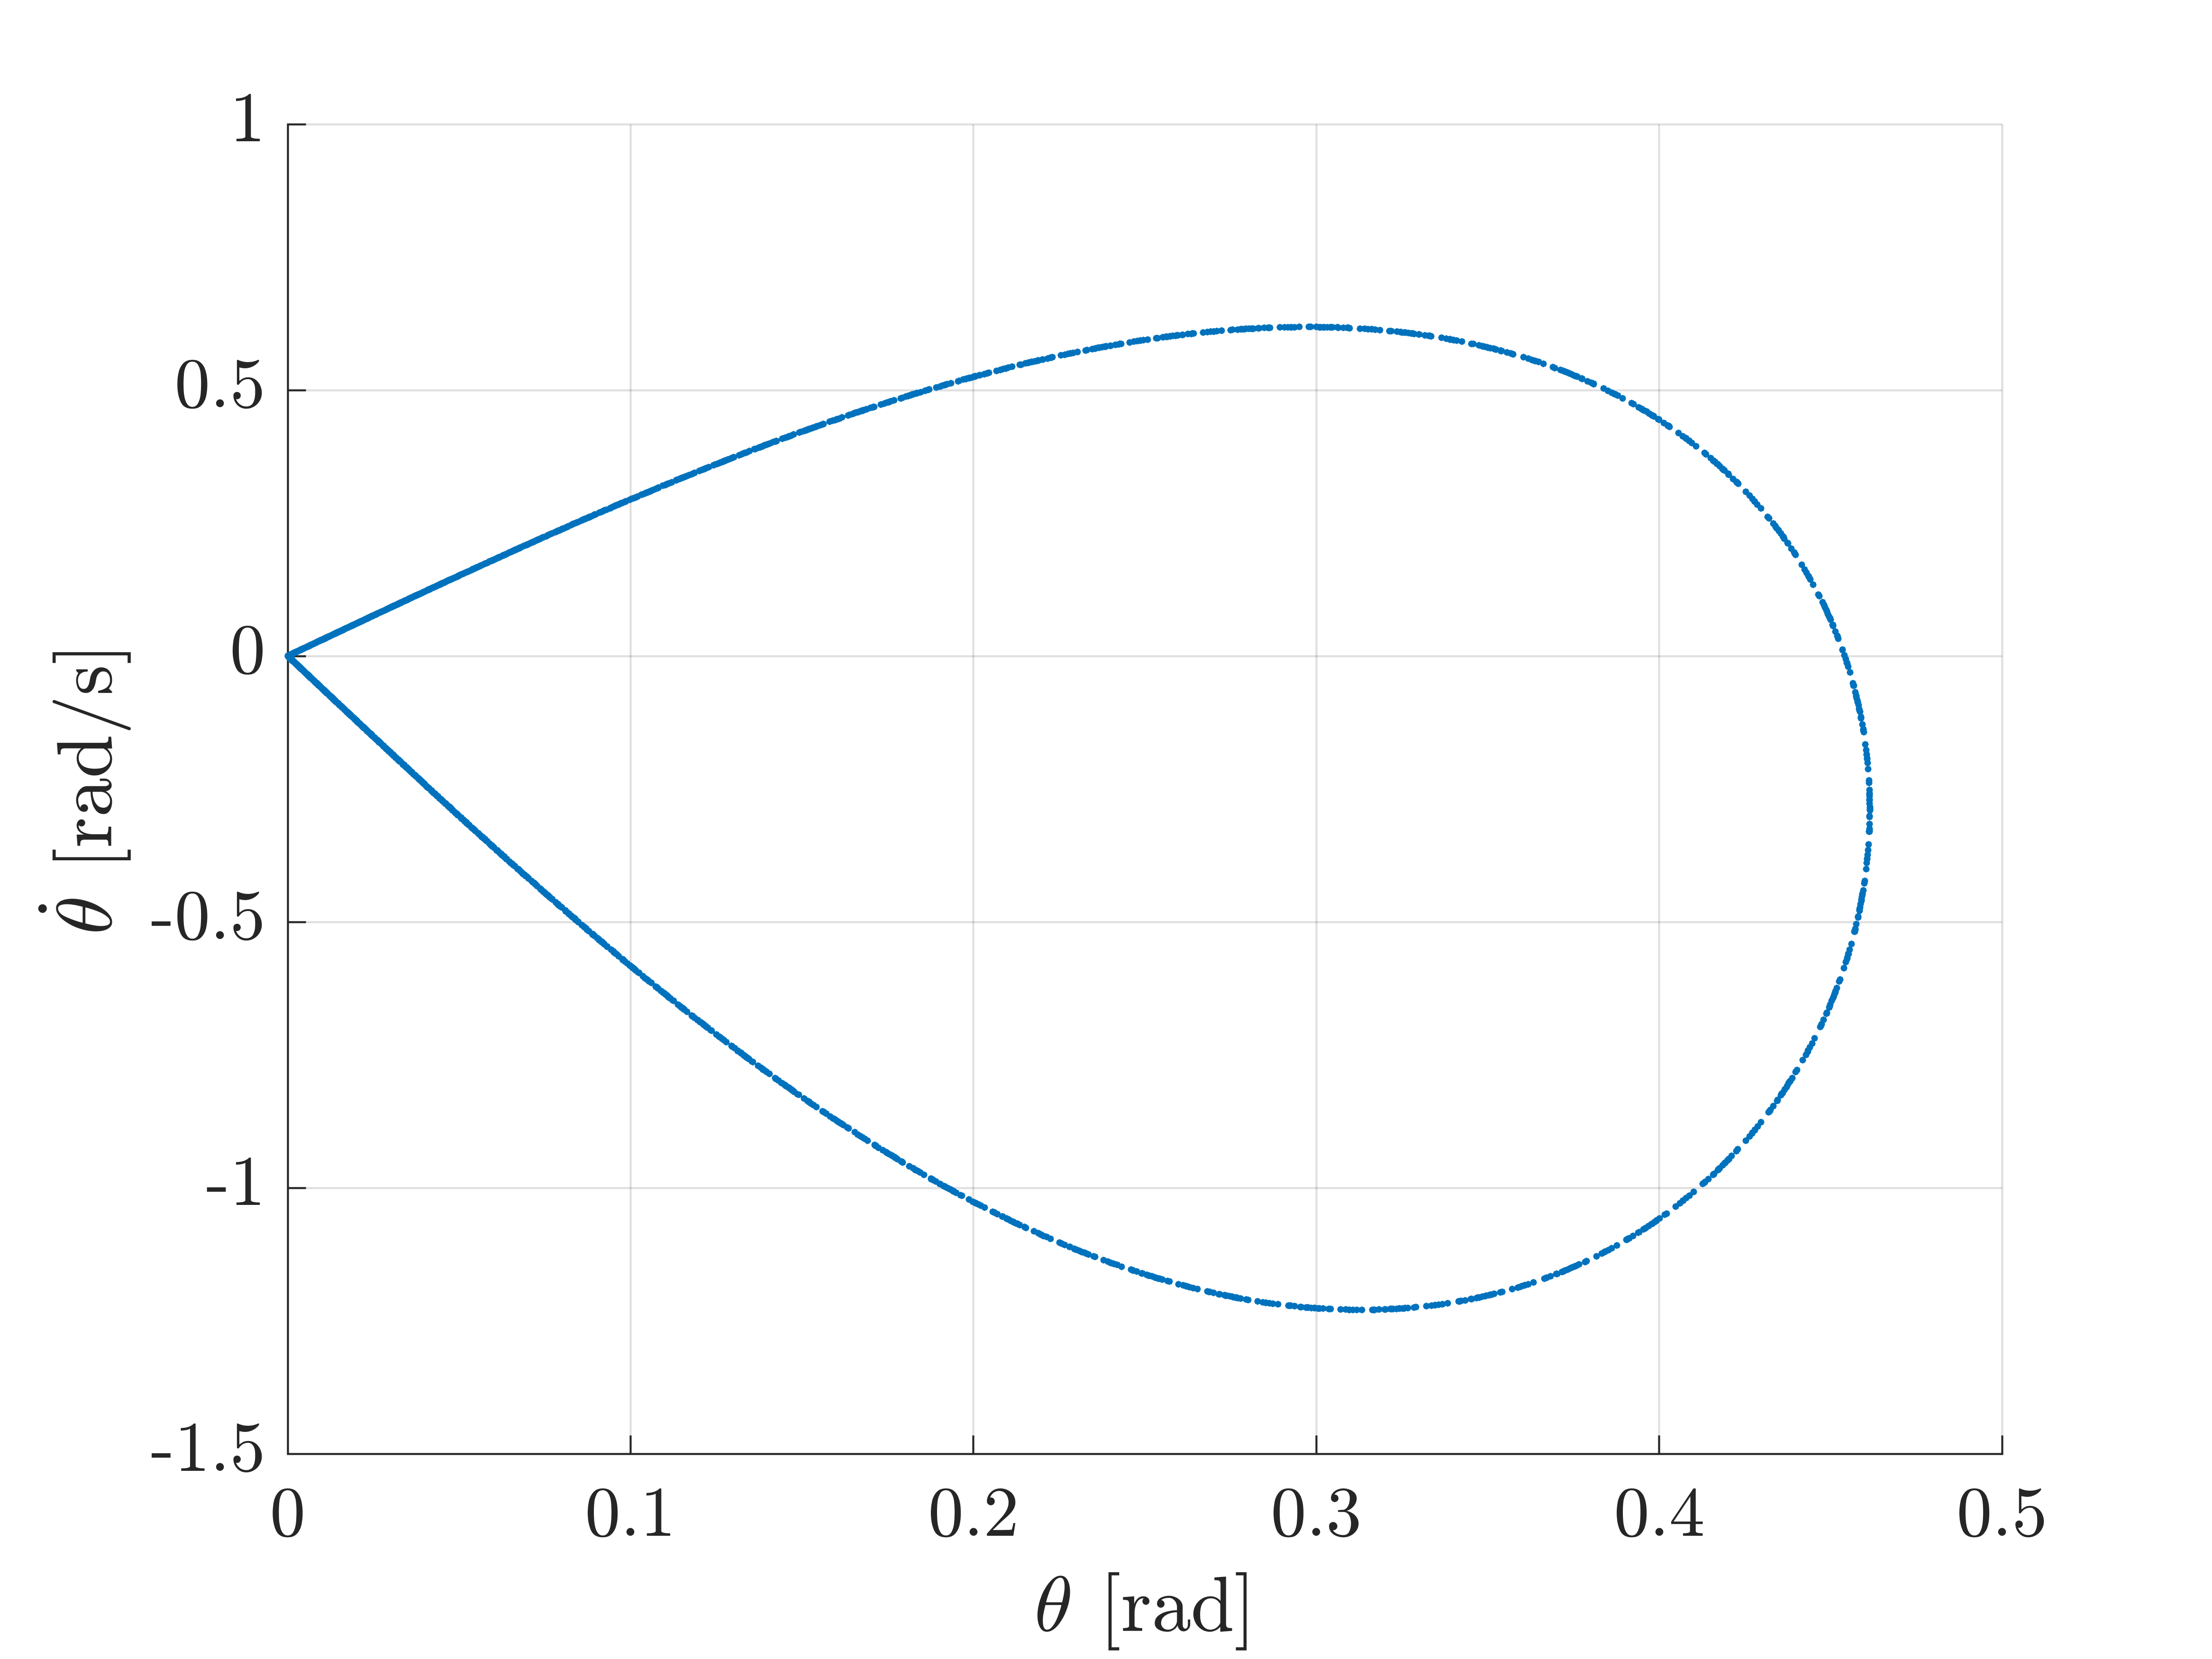
\includegraphics[width=\textwidth]{graphs/e_poincare_drop.png}
		\caption{Non-chaotic simulation of initial conditions: $\theta_0 = \SI{1e-6}{\radian}$ and $\dot{\theta_0}=\SI{0}{\radian\per\s}$.}
		\label{fig:e-pc-drop}
	\end{subfigure}
	\caption{Set of sections of poincaré, all with the number of steps for each period taken at $n=100$, an simulation time given by $t_{end} \approx \SI{6344}{\s}$ and $dt \approx \num{6.3d-3} s$.}
	\label{fig:e-pc}
\end{figure}

Figures \ref{fig:e-pc-MK8}, \ref{fig:e-pc-peanut} and \ref{fig:e-pc-drop} are non-chaotic simulation of the pendulum.
It is non-chaotic, because the trajectory in the phase space remains the same over time, which means that it is possible to predict the position of the pendulum at any time.
On the other hand, \ref{fig:e-pc-chaos1} is a chaotic simulation of the pendulum.
This time, the trajectory in the phase space is a set of points vaguely following a thick path, which means that after a moment, the position of the pendulum can not be predicted.

\subsubsection{Sensitivity on initial condition}

\begin{figure}[h]
\centering
	\begin{subfigure}[t]{0.47\textwidth}
		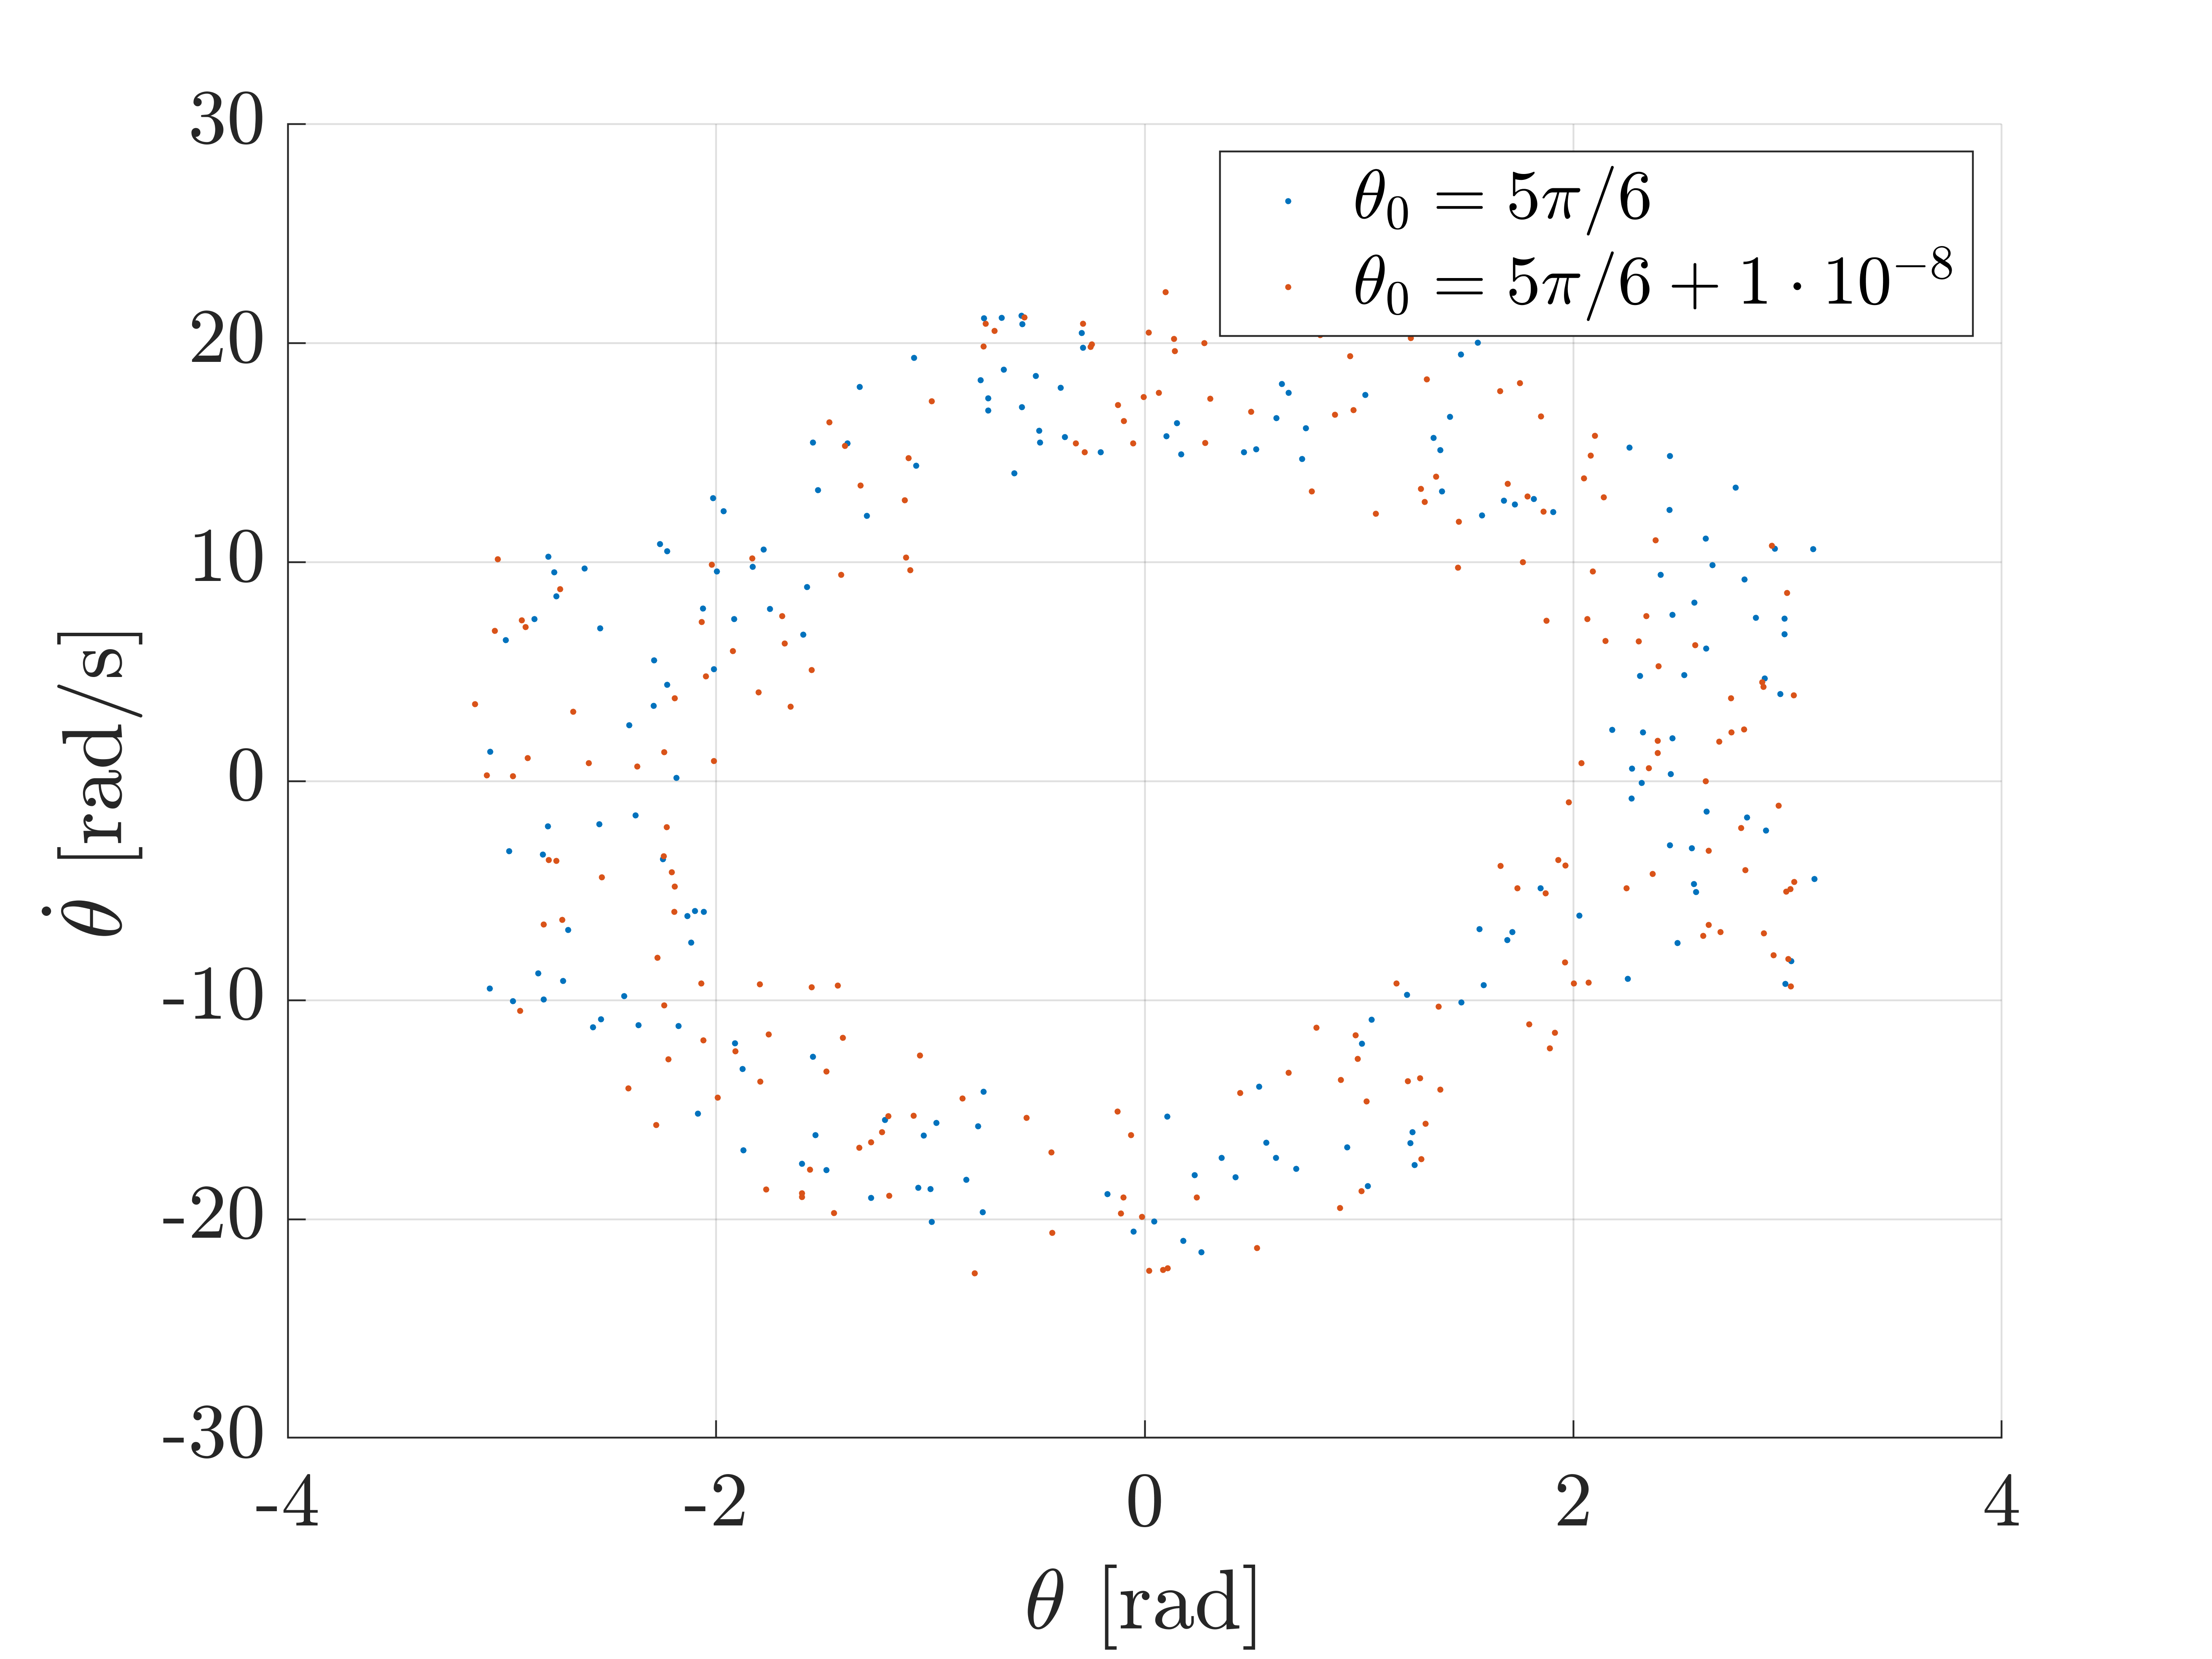
\includegraphics[width=\textwidth]{graphs/e_sens_chaos.png}
		\caption{Poincaré section of two chaotic simulations}
		\label{fig:e-sens-chaos}
	\end{subfigure}
	~
	\begin{subfigure}[t]{0.45\textwidth}
		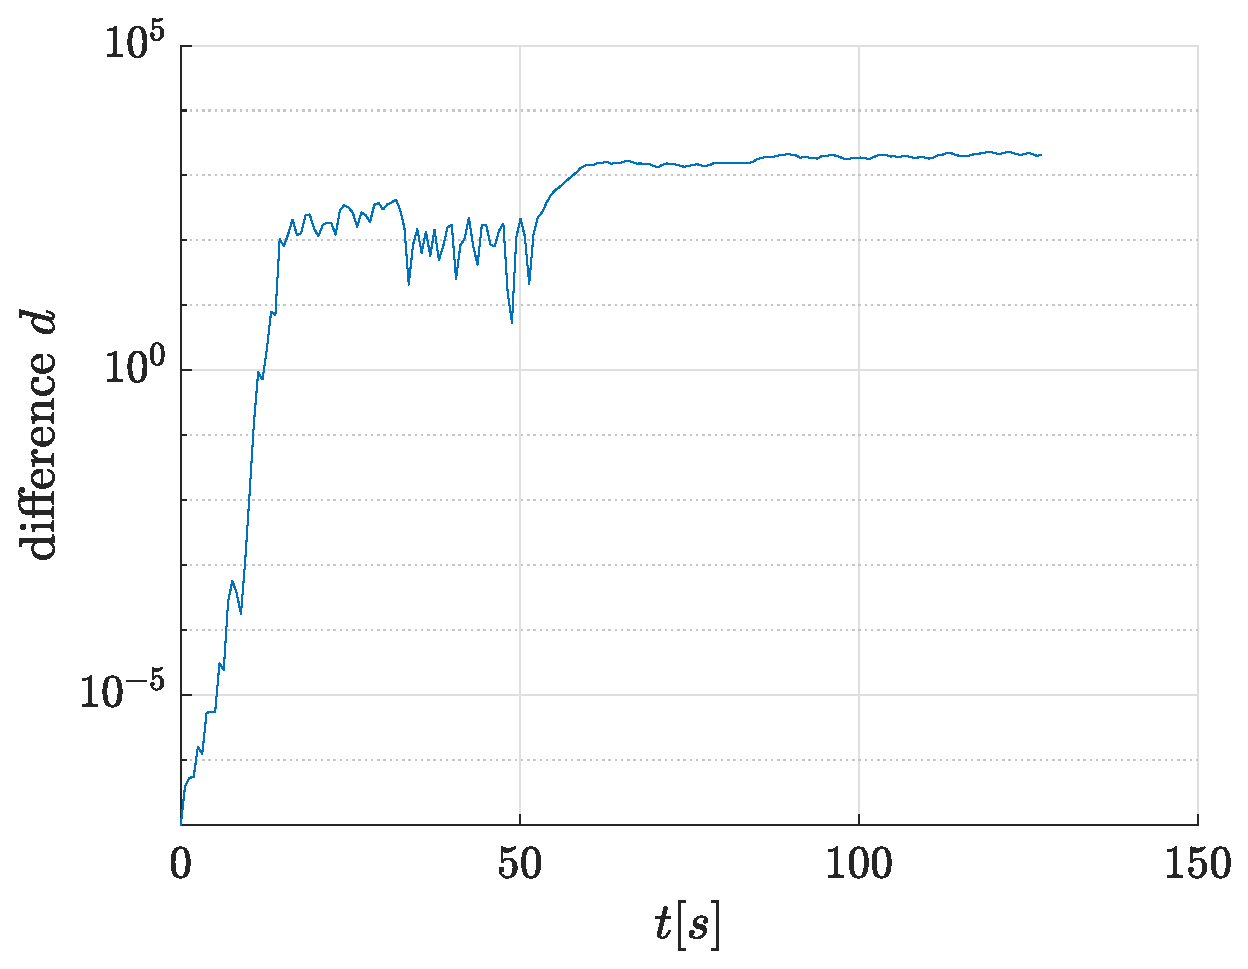
\includegraphics[width=\textwidth]{graphs/e_lyap_chaos.eps}
		\caption{Difference of two chaotic simulations over time}
		\label{fig:e-lyap-chaos}
	\end{subfigure}
	\caption{Comparison of two chaotic simulations with an initial angle difference of \num{1d-8} and initial velocity $\theta_0 = 0$}
	\label{fig:e-chaos}
\end{figure}

Figure \ref{fig:e-chaos} was made with the number of steps for each period $n=500$, the final time $t_{end} \approx 127 s$ and a time step of $dt \approx \num{1.3d-2} s$. As expected of chaos, we get two different distributions of points for the Poincaré section, although they are both distributed over the same general area. Figure \ref{fig:e-lyap-chaos} shows the difference between the two simulations over time, calculated as $d=\sqrt{(\dot{\theta_1}-\dot{\theta_2})^2 + \Omega^2 (\theta_1-\theta_2)^2}$. From this graph we can calculate the Lyapunov exponent $\lambda$, which is the slope of $log(d(t))$ in the initial phase of the simulation. With $t_0 = 0$ initially and $t_1=14.59$ at the top of the slope, we get:
\begin{equation*}
\lambda = \frac{d(t_1)-d(t_0)}{t_1-t_0} \approx 7.14
\end{equation*}
The Lyapunov exponent characterizes the rate of separation in the phase space between infinitesimally close dynamical systems.\cite{Lyap} In this case, as $\lambda > 0$, it indicates a chaotic system.\cite{Lyap2}

\begin{figure}[h]
\centering
	\begin{subfigure}[t]{0.47\textwidth}
		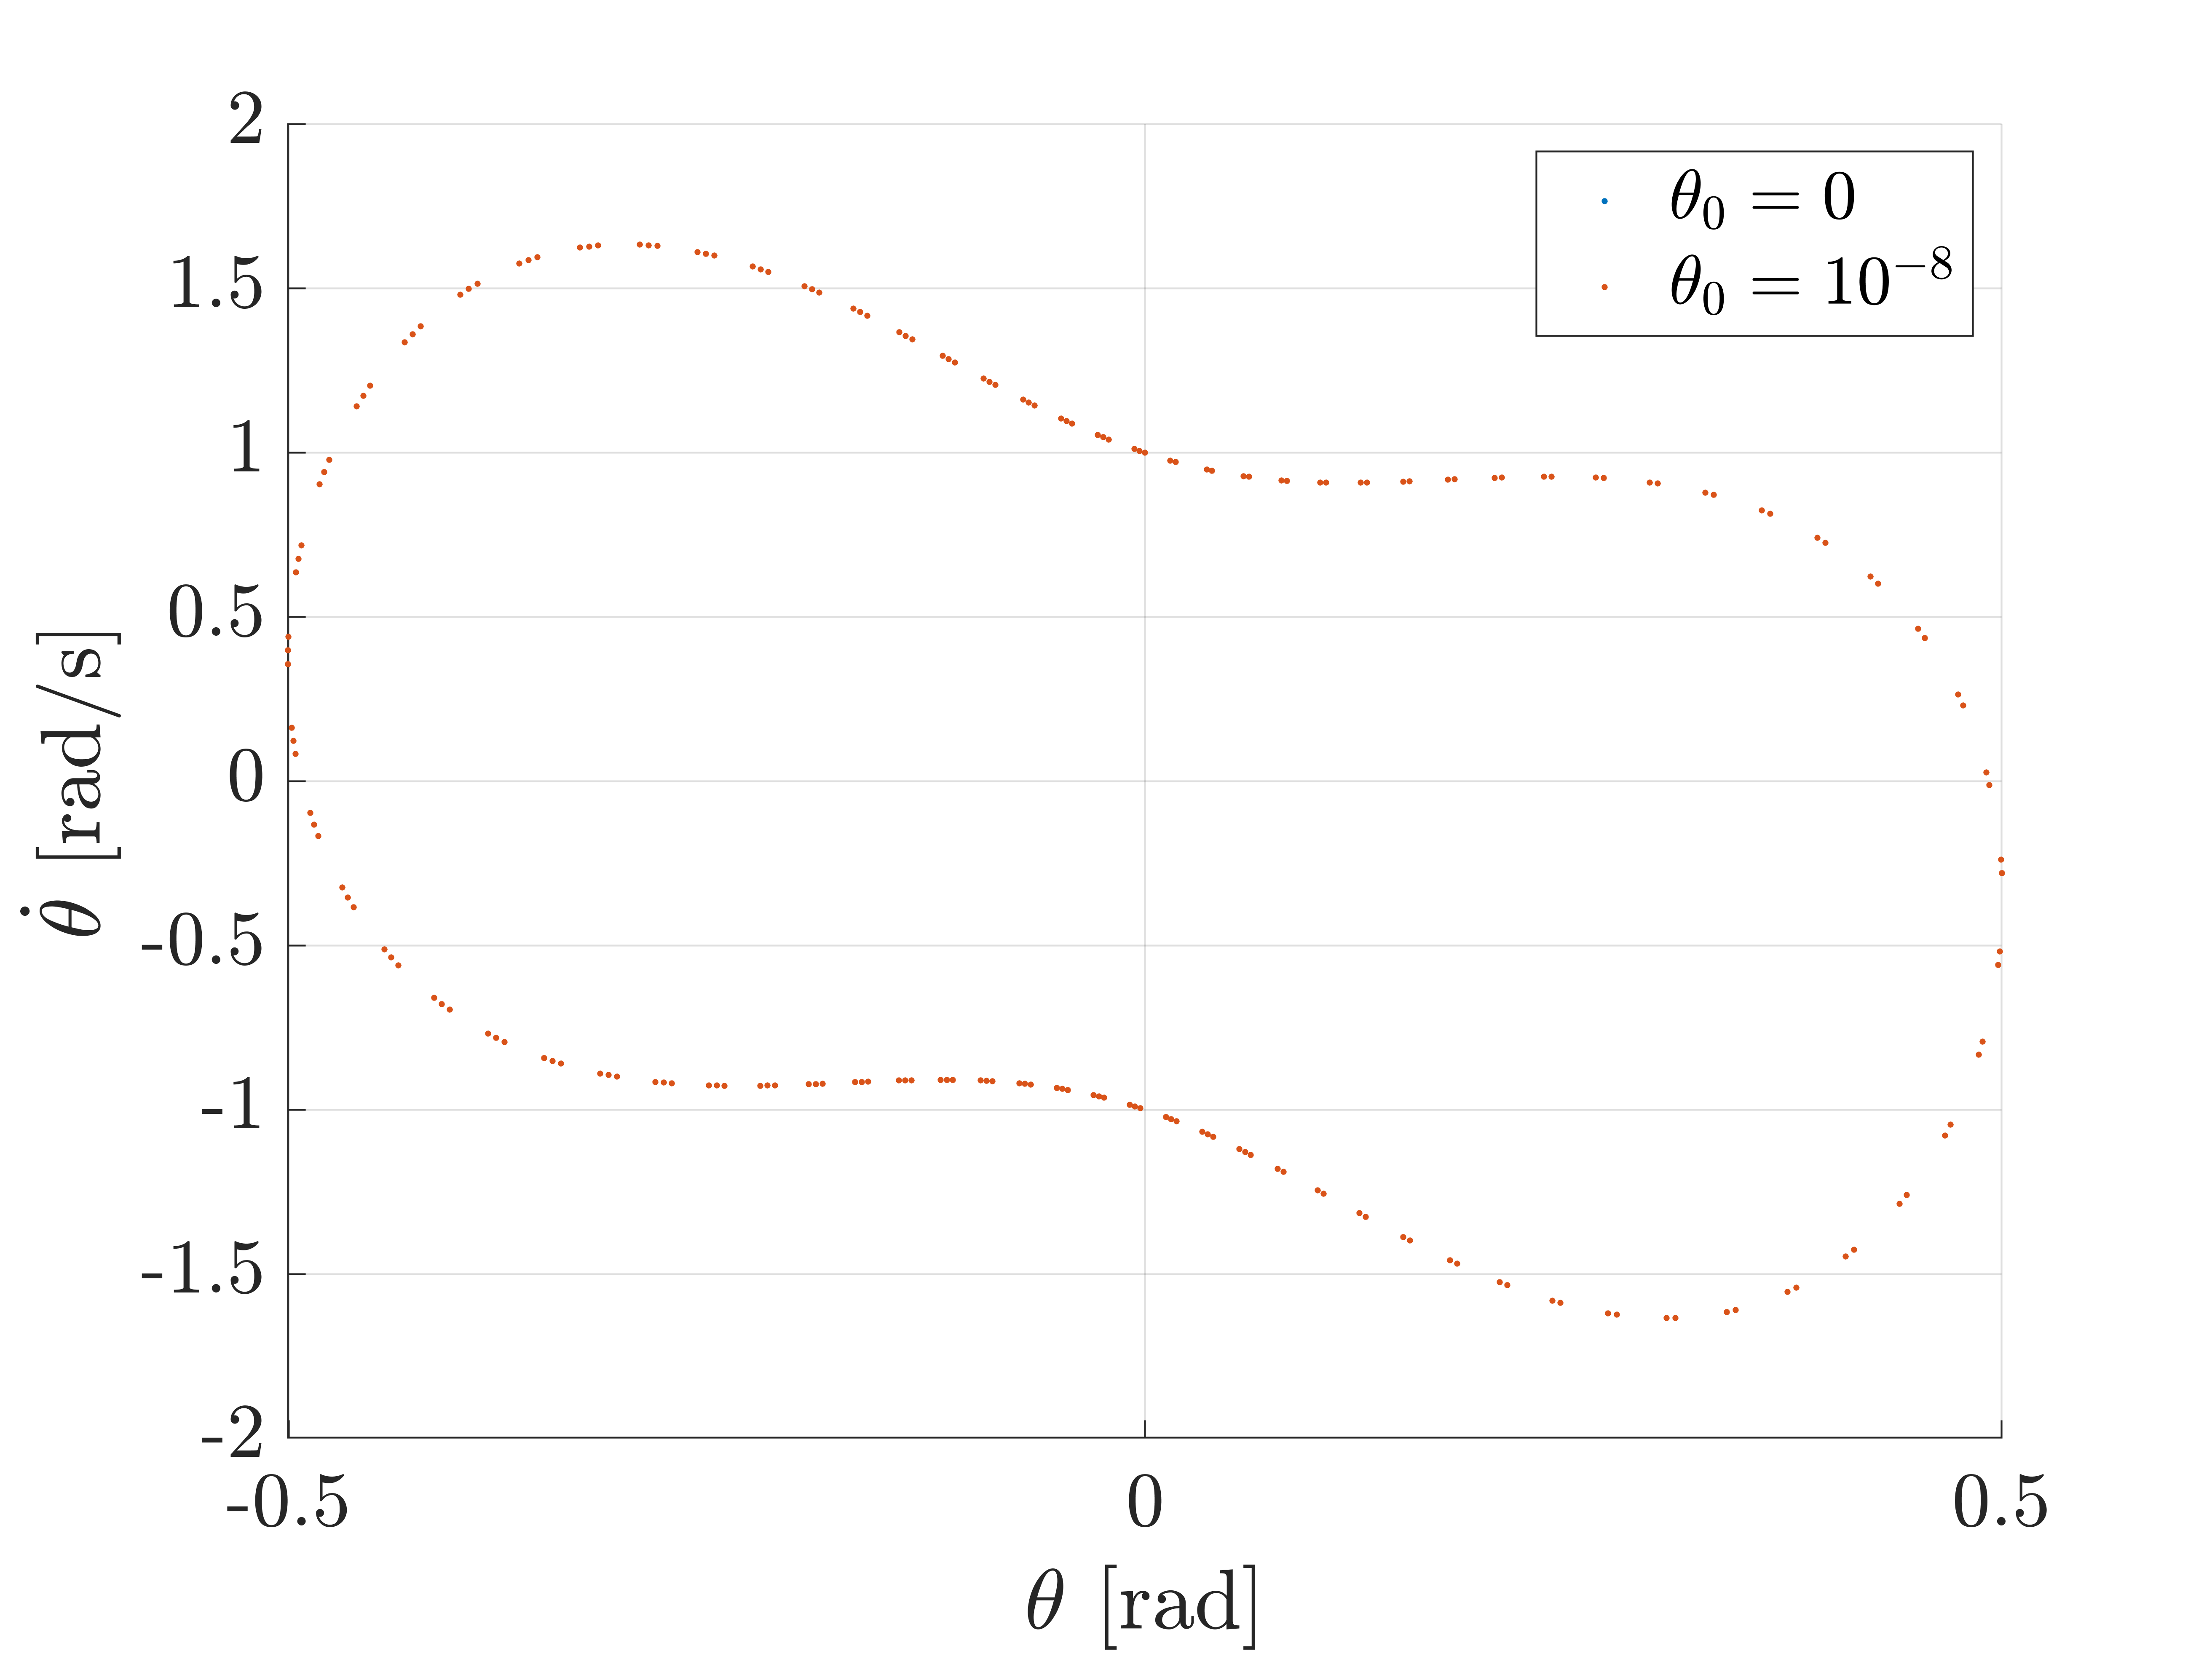
\includegraphics[width=\textwidth]{graphs/e_sens_notchaos.png}
		\caption{Poincaré section of two stable simulations}
		\label{fig:e-sens-notchaos}
	\end{subfigure}
	~
	\begin{subfigure}[t]{0.45\textwidth}
		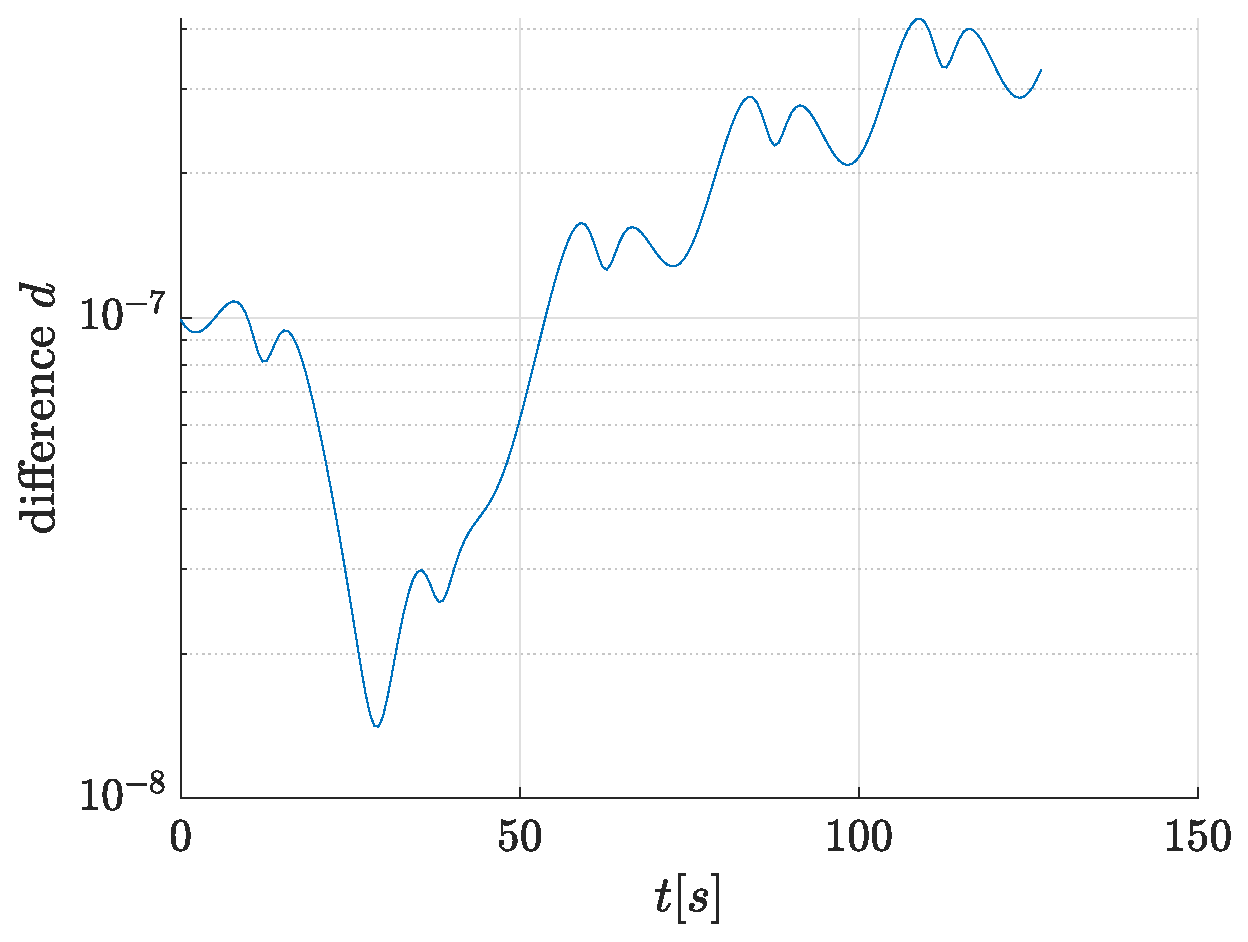
\includegraphics[width=\textwidth]{graphs/e_lyap_notchaos.eps}
		\caption{Difference of two stable simulations over time}
		\label{fig:e-lyap-notchaos}
	\end{subfigure}
	\caption{Comparison of two stable simulations with an initial angle difference of \num{1d-8} and initial velocity $\theta_0 = 1$}
	\label{fig:e-notchaos}
\end{figure}

Figure \ref{fig:e-notchaos} was made with the same numerical conditions as figure \ref{fig:e-chaos}, for a stable system. In this case, an infinitesimally small difference on the initial position does not cause any significant divergence between the two systems over the course of the simulation, as their Poincaré sections are superimposed. We can once again calculate the Lyapunov exponent from the initial slope of figure \ref{fig:e-lyap-notchaos}, with $t_0 = 0$ and $t_1=29.18$:
\begin{equation*}
\lambda \approx \num{-2.91d-9}
\end{equation*}
As $\lambda < 0$, it indicates a stable system.\cite{Lyap2}

%%%%%%%%%%%%%%%%%%%%%%%%%%%%%%%%%

\subsection{Poincaré section: chaos with air resistance}


\subsection{Optional} %TODO : Changer le titre.

\begin{thebibliography}{99}
	\bibitem{wiki:en-cin} Énergie mécanique. (2018, September 14). Wikipédia, l'encyclopédie libre. Retrieved 16:51, September 14, 2018 from \url{http://fr.wikipedia.org/w/index.php?title=%C3%89nergie_m%C3%A9canique&oldid=152194224}.
	\bibitem{Lyap} Wikipedia contributors. (2018, October 6). Lyapunov exponent. In Wikipedia, The Free Encyclopedia. Retrieved 08:56, November 18, 2018, from \url{https://en.wikipedia.org/w/index.php?title=Lyapunov_exponent&oldid=862716940}
	\bibitem{Lyap2} 4.3 Lyapunov Exponent. The Chaos Hypertextbook. Retrieved 09:58, September 14, 2018 from \url{https://hypertextbook.com/chaos/lyapunov-1/}

\end{thebibliography}

\end{document}
